%\documentclass[journal]{vgtc}                % final (journal style)
\documentclass[review,journal]{vgtc}         % review (journal style)
%\documentclass[widereview]{vgtc}             % wide-spaced review
%\documentclass[preprint,journal]{vgtc}       % preprint (journal style)

%% Uncomment one of the lines above depending on where your paper is
%% in the conference process. ``review'' and ``widereview'' are for review
%% submission, ``preprint'' is for pre-publication, and the final version
%% doesn't use a specific qualifier.

%% Please use one of the ``review'' options in combination with the
%% assigned online id (see below) ONLY if your paper uses a double blind
%% review process. Some conferences, like IEEE Vis and InfoVis, have NOT
%% in the past.

%% Please use the ``preprint''  option when producing a preprint version
%% for sharing your article on an open access repository

%% Please note that the use of figures other than the optional teaser is not permitted on the first page
%% of the journal version.  Figures should begin on the second page and be
%% in CMYK or Grey scale format, otherwise, colour shifting may occur
%% during the printing process.  Papers submitted with figures other than the optional teaser on the
%% first page will be refused. Also, the teaser figure should only have the
%% width of the abstract as the template enforces it.

%% These few lines make a distinction between latex and pdflatex calls and they
%% bring in essential packages for graphics and font handling.
%% Note that due to the \DeclareGraphicsExtensions{} call it is no longer necessary
%% to provide the the path and extension of a graphics file:
%% 
\includegraphics{diamondrule} is completely sufficient.
%%
\ifpdf%                                % if we use pdflatex
  \pdfoutput=1\relax                   % create PDFs from pdfLaTeX
  \pdfcompresslevel=9                  % PDF Compression
  \pdfoptionpdfminorversion=7          % create PDF 1.7
  \ExecuteOptions{pdftex}
  \usepackage{graphicx}                % allow us to embed graphics files
  \DeclareGraphicsExtensions{.pdf,.png,.jpg,.jpeg} % for pdflatex we expect .pdf, .png, or .jpg files
\else%                                 % else we use pure latex
  \ExecuteOptions{dvips}
  \usepackage{graphicx}                % allow us to embed graphics files
  \DeclareGraphicsExtensions{.eps}     % for pure latex we expect eps files
\fi%

%% it is recomended to use ``\autoref{sec:bla}'' instead of ``Fig.~\ref{sec:bla}''
\graphicspath{{figs/}{pictures/}{images/}{./}} % where to search for the images

\usepackage{microtype}                 % use micro-typography (slightly more compact, better to read)
\PassOptionsToPackage{warn}{textcomp}  % to address font issues with \textrightarrow
\usepackage{textcomp}                  % use better special symbols
\usepackage{mathptmx}                  % use matching math font
\usepackage{times}                     % we use Times as the main font
\renewcommand*\ttdefault{txtt}         % a nicer typewriter font
\usepackage{cite}                      % needed to automatically sort the references
\usepackage{tabu}                      % only used for the table example
\usepackage{booktabs}                  % only used for the table example
%% We encourage the use of mathptmx for consistent usage of times font
%% throughout the proceedings. However, if you encounter conflicts
%% with other math-related packages, you may want to disable it.

% \setlength{\textfloatsep}{0.3\baselineskip plus 0.1\baselineskip minus 0.3\baselineskip}
\setlength{\textfloatsep}{0.1\baselineskip}

%% Regulus specific packages
\usepackage{scrextend}
\usepackage{enumitem}
\usepackage{todonotes}

% \usepackage{titlesec}
% \titlespacing{\section}{0pt}{*2}{*1}
% \titlespacing*{\section}
% {0pt}{2\baselineskip}{3\baselineskip}
% \titlespacing*{\subsection}
% {0pt}{5.5ex plus 1ex minus .2ex}{4.3ex plus .2ex}

% Select what to do with command \comment:
% \newcommand{\comment}[1]{}  %comment not showed
\newcommand{\comment}[2]
{\par {\bfseries \color{blue} [#2]: #1 \par}} %comment showed

\usepackage{algorithm}
\usepackage[noend]{algpseudocode}
\usepackage{listings}
\usepackage{xcolor}

\newcommand{\regulus}{\emph{Regulus}~}
\newcommand{\RT}{Regulus Tree~}
\newcommand{\MSC}{More-Smale complex~}

%New colors defined below
\definecolor{codegreen}{rgb}{0,0.6,0}
\definecolor{codegray}{rgb}{0.5,0.5,0.5}
\definecolor{codepurple}{rgb}{0.58,0,0.82}
\definecolor{backcolour}{rgb}{0.95,0.95,0.92}

%Code listing style named "mystyle"
\lstdefinestyle{mystyle}{
% backgroundcolor=\color{backcolour},
  commentstyle=\color{codegreen},
  keywordstyle=\color{magenta},
  numberstyle=\tiny\color{codegray},
  stringstyle=\color{codepurple},
  basicstyle=\ttfamily\footnotesize,
  breakatwhitespace=false,
  breaklines=true,
  captionpos=b,
  frame=single,
  keepspaces=true,
%   numbers=left,
%   numbersep=5pt,
  showspaces=false,
  showstringspaces=false,
  showtabs=false,
  tabsize=2
}
%"mystyle" code listing set
\lstset{style=mystyle}

%% In preprint mode you may define your own headline. If not, the default IEEE copyright message will appear in preprint mode.
%\preprinttext{To appear in IEEE Transactions on Visualization and Computer Graphics.}

%% In preprint mode, this adds a link to the version of the paper on IEEEXplore
%% Uncomment this line when you produce a preprint version of the article
%% after the article receives a DOI for the paper from IEEE
%\ieeedoi{xx.xxxx/TVCG.201x.xxxxxxx}

%% If you are submitting a paper to a conference for review with a double
%% blind reviewing process, please replace the value ``0'' below with your
%% OnlineID. Otherwise, you may safely leave it at ``0''.
\onlineid{1155}

%% declare the category of your paper, only shown in review mode
\vgtccategory{Research}
%% please declare the paper type of your paper to help reviewers, only shown in review mode
%% choices:
%% * algorithm/technique
%% * application/design study
%% * evaluation
%% * system
%% * theory/model
\vgtcpapertype{algorithm/technique}

%% Paper title.
\title{A Novel Tree Visualization to Guide Interactive Exploration of Multi-dimensional Topological Hierarchies}

%% This is how authors are specified in the journal style

%% indicate IEEE Member or Student Member in form indicated below
\author{Yarden Livnat%, \textit{Member, IEEE}
	, Dan Maljovec
	, Attila Gyulassy,
	, Baptiste Mouginot,
	, Valerio Pascucci
	}
\authorfooter{
%% insert punctuation at end of each item
\item
 Yarden Livnat is with the Scientific Computing and Imaging Institute at the University of Utah.
 E-mail: yarden@sci.utah.edu.
\item
 Dan Maljovec is with the xxx.
 E-mail: maljovec@sci.utah.edu
 \item  Attila Gyulassy is with xxx.
 E-mail: attila.gyulassy@gmail.com.
 \item  Baptiste Mouginot is with Nuclear Engineering department at the University of Wisconsin-Madison.
 E-mail: mouginot@wisc.edu.
 \item
 Valerio Pascucci is with the Scientific Computing and Imaging Institute at the University of Utah.
 E-mail: pascucci@sci.utah.edu.
}

%other entries to be set up for journal
\shortauthortitle{Livnat \MakeLowercase{\textit{et al.}}: A Novel Dynamic Tree Layout for Visual Exploration of Multi-dimensional Topological Hierarchies}
%\shortauthortitle{Firstauthor \MakeLowercase{\textit{et al.}}: Paper Title}

%% Abstract section.
\abstract{Understanding the response of an output variable to multi-dimensional inputs lies at the heart of many data exploration endeavours. Topology-based methods, in particular Morse theory and persistent homology, provide a useful framework for studying this relationship, as phenomena of interest often appear naturally as fundamental features. The Morse-Smale complex captures a wide range of features by partitioning the domain of a scalar function into piecewise monotonic regions, while persistent homology provides a means to study these features at different scales of simplification. Previous works demonstrated how to compute such a representation and its usefulness to gain insight into multi-dimensional data. However, exploration of the multi-scale nature of the data was limited to selecting a single simplification threshold from a plot of region count. In this paper, we present a novel tree visualization that provides a concise overview of the entire hierarchy of topological features. The structure of the tree provides initial insights in terms of the distribution, size, and stability of all partitions. We use regression analysis to fit linear models in each partition, and develop local and relative measures to further assess uniqueness and the importance of each partition, especially with respect parents/children in the feature hierarchy. The expressiveness of the tree visualization becomes apparent when we encode such measures using colors, and the layout allows an unprecedented level of control over feature selection during exploration. For instance, selecting features from multiple scales of the hierarchy enables a more nuanced exploration. Finally, we demonstrate our approach using examples from several scientific domains.
%
%Morse-Smale theory and persistence homology form a rich and powerful topology-based framework for studying complex high-dimensional scalar functions. A Morse-Smale complex captures a wide range of features by decomposing the scalar function into piecewise monotonic partitions while persistence homology provides a means for simplifying it at different levels of detail. Previous works focused on \textit{how} to create a simplified topological description for a given persistence value but provided only crude measures to help a user select an appropriate value from  ordered list of persistence values. 
%In this paper, we present a novel tree visualization that provides a concise hierarchical overview of all simplification steps with respect to their persistence levels. The overall structure of the tree provides initial insights in terms of the distribution, size and stability of all potential space partitioning. Rather than relying only on topological attributes, we use regression analysis to fit linear models in all potential partitions and develop local and relative measures to further assess uniqueness and the importance of each partition. The expressiveness of the tree visualization becomes apparent when we encode measures using colors and interact with one or more trees to guide the exploration of simplification space and the underlying function, and identify partitions of unique behavior. In addition, we discuss the notions of local and non-consistent simplifications using partitions from different persistence levels. Finally, we demonstrate our approach using examples from several scientific domains.
} 


%% Keywords that describe your work. Will show as 'Index Terms' in journal
%% please capitalize first letter and insert punctuation after last keyword
\keywords{Computational Topology-based Techniques, High-dimensional Data, Data Models, Graph/Network and Tree Data. Multi-Resolution and Level of Detail Techniques.
% Multidimensional data, Topology, Data exploration.
}

%% ACM Computing Classification System (CCS).
%% See <http://www.acm.org/class/1998/> for details.
%% The ``\CCScat'' command takes four arguments.

%\CCScatlist{ % not used in journal version
% \CCScat{K.6.1}{Management of Computing and Information Systems}%
%{Project and People Management}{Life Cycle};
% \CCScat{K.7.m}{The Computing Profession}{Miscellaneous}{Ethics}
%}

%% A teaser figure can be included as follows
\teaser{
  \centering
  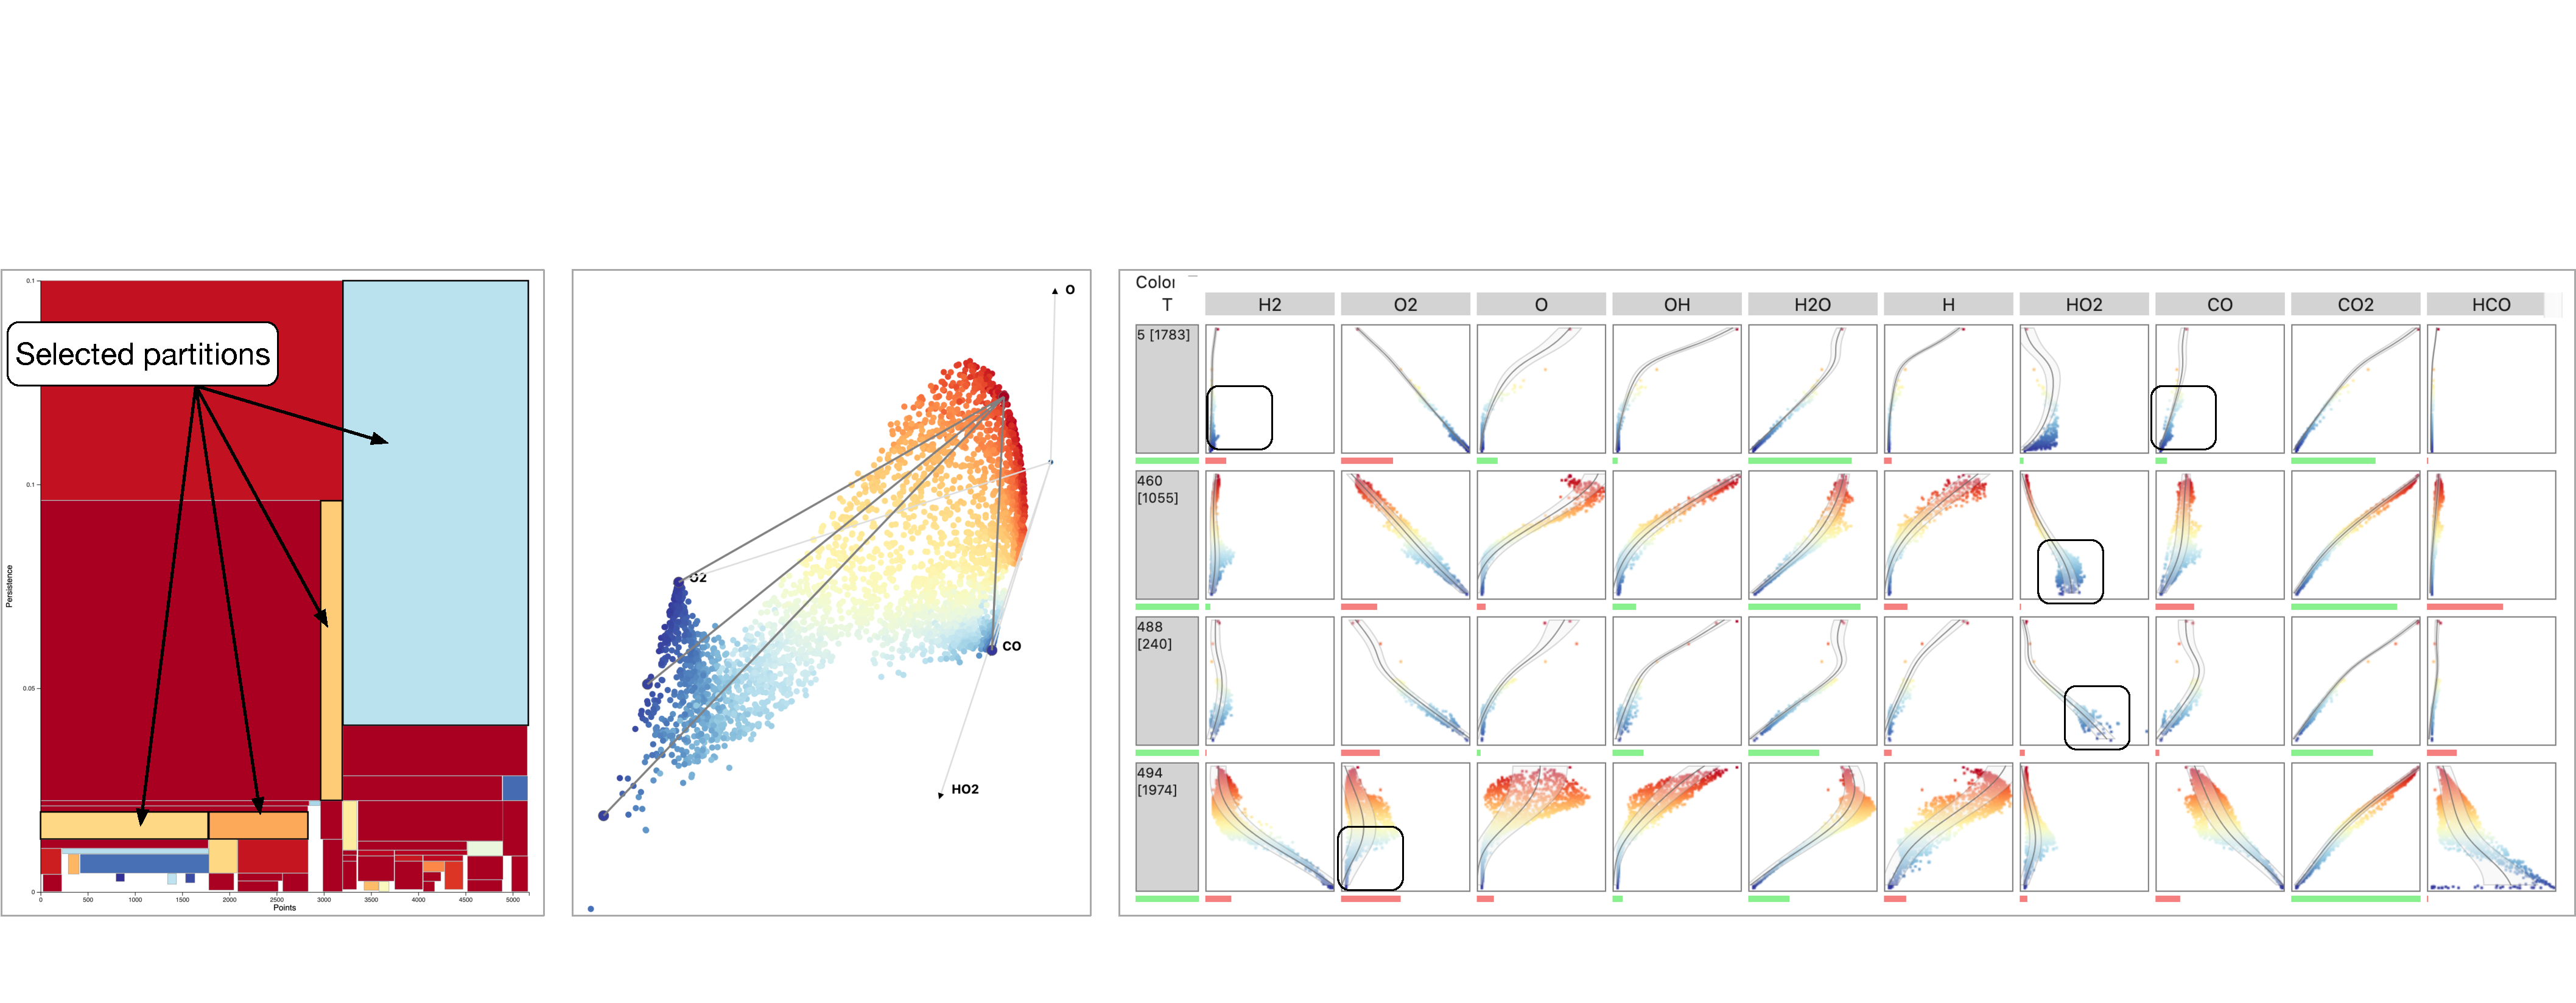
\includegraphics[width=\linewidth]{figs/teaser-3}
  \caption{A \RT provides a concise annotated overview of all Morse-Smale complex partitions for the entire persistence hierarchy. In a study of temperature as a function of chemical species, the \RT on the left encodes Child Dimension Fitness that highlights partitions with different characteristics than their parents (red/blue indicate small/large differences).  Selection of the top partitions shows a single maximum and four distinct minima in the graph view (middle). Projections of the data points in the four partitions (right) demonstrates that two unique minima are due to lack of fuel (top) and lack of oxidizer (bottom), while the other two identify  unmixed fuel and oxidizer due to turbulence in the combustion reaction. }
  \label{fig:teaser}
}

%% Uncomment below to disable the manuscript note
%\renewcommand{\manuscriptnotetxt}{}

%% Copyright space is enabled by default as required by guidelines.
%% It is disabled by the 'review' option or via the following command:
% \nocopyrightspace


\vgtcinsertpkg

%%%%%%%%%%%%%%%%%%%%%%%%%%%%%%%%%%%%%%%%%%%%%%%%%%%%%%%%%%%%%%%%
%%%%%%%%%%%%%%%%%%%%%% START OF THE PAPER %%%%%%%%%%%%%%%%%%%%%%
%%%%%%%%%%%%%%%%%%%%%%%%%%%%%%%%%%%%%%%%%%%%%%%%%%%%%%%%%%%%%%%%%

\begin{document}

%% The ``\maketitle'' command must be the first command after the
%% ``\begin{document}'' command. It prepares and prints the title block.

%% the only exception to this rule is the \firstsection command
%\firstsection{Introduction}

%\maketitle

%% \section{Introduction} %for journal use above \firstsection{..} instead
%This template is for papers of VGTC-sponsored conferences such as IEEE VIS, IEEE VR, and ISMAR which are published %as special issues of TVCG. The template does not contain the respective dates of the conference/journal issue, these %will be entered by IEEE as part of the publication production process. Therefore, \textbf{please leave the copyright %statement at the bottom-left of this first page untouched}.
%

\firstsection{Introduction}
\maketitle
\label{sec:intro}

Many phenomena in science and engineering can be described by how an output variable depends on input parameters. For example, understanding the correlation between temperature and chemical species and turbulence in a computationally model of a combustion reaction can lead to better fuel or engine designs. As another example, understanding how the measured strength of concrete varies with the ratios of its ingredients can lead to more error-tolerant mixtures. Computational models are used to study such real-world phenomena, either by conducting computer simulations or through a set of well-designed experiments. Analysis of the results can then be used to improve the models, find optimal solutions, uncover unknown relationships, and support decision-making.

The set of relationships between inputs and output can be very specialized; for any input parameter, its relationship to the output variable may be conditioned on the variation in the other parameters. Topology provides a means of studying the shape of a function; for instance, identifying how local minima and maxima are related to each other both spatially and in terms of local importance. The Morse-Smale complex, in particular, decomposes the domain into monotonic regions that enable reasoning about local trends that contribute to the formation of a local maximum or minimum. In contrast to a user-defined query or hypercube sample, the topological partitions are intrinsic to the function and underlying manifold, and are well-suited for regression analysis. 

Local perturbations, artifacts of meshing, or small features can derail analysis, as it is difficult to separate phenomena from noise. Persistent homology describes topological features in terms of their life-span of the element from its birth critical point to its death in a sweep of the range of the function. In many applications, features below a persistence threshold are discarded as noise, a process that involves guesstimating an appropriate value, sometimes with the help of a persistence curve. In many applications, however, features appear with varying persistence in the domain. In multi-dimensional data analysis, in particular, justifying a simplification threshold is difficult as, until now, there have not been effective visualization and exploration techniques to understand the specific relationships between features at different scales. 

We introduce a novel visualization that is composed of a nested space-filling tree layout to visualize the topological hierarchy whose geometry encodes the size and persistence of topological features. We reinterpret persistence simplification hierarchies of the Morse-Smale complex as a merging tree of partitions, allowing an even finer granularity of feature selection than a single simplification operation and efficient layout. Color in the cells of the tree is used to encode one of many computed measures, such as fitness of a regression model to the corresponding topological feature, relationships between the models of parents and children, or any other computed attributes. Our new visualization is deployed in an open exploration environment implemented in Python and JupyterLab extensions. Linked views enable dynamic feature selection for flexible analysis. We evaluate the utility of the approach with use cases in combustion and nuclear energy, where salient features are visible at a glance, that previously depended on an exhaustive search through the simplification parameter.
Specifically, our contributions are:
\begin{itemize}[nosep]
    \item A new interpretation of persistence simplification of a Morse-Smale complex as a merger tree of partitions,

    \item A new visualization of topological hierarchies that encodes the size and life-span of every feature at once,

    \item Measures on topological features that incorporate the ancestry of a partition to aid and guide users in selecting the topological scale for analysis, 

    \item A user interface that enables adaptive simplification, and non-uniform and non-consistent selection of features across multiple scales, 
    
    \item Design of an open exploration environment to facilitate exploratory analysis. 
\end{itemize}


% \begin{itemize}[topsep=0cm, itemsep=0ex, parsep=0cm]
%     \item Computational models are used to study real-world phenomena, either by conducting computer simulations or a set of well-designed experiments. Give examples.
    
%     \item Analysis of the results can then be used to improve the models, find optimal solutions, uncover unknown relationships and support decision-making.
        
%     \item One important aim is to understand the shape of the output function. What are the local min and max values, where are they located and how are they associated with each other. Where are the min and max, how stable the function is at various location.
    
%     \item Another important aspect is understanding the behaviour of the function, that is the relationship between the input parameters and the output.
    
%     \item In particular, identifying regions of interest where the output function has unique characteristics or behavior with respect to the input parameters. Understanding the characteristics of the function in these ROI and around certain critical points.
    
%     \item These analysis can be done on the output function or on derived quantities.
    
%     \item Topology
    
%     \begin{itemize}
%         \item Morse-Smale and hierarchical simplification to deal with noise.
        
%          \item Geometric Skeleton: inverse relationships indicating which combinations of inputs are responsible for which output.
     
%         \item Topology data analysis (or is it Morse-Smale approaches?) tools often focus on on extrapolating $f$ at various refinement levels.
%     \end{itemize}

%     \item Simulation Ensembles
%     \todo[inline]{maybe this shouldn't be in the paper}

% \end{itemize}

% \item In this paper we focus on scalar functions. We use MSC theory to define local approximation of the function rather than a complete global one. 

% \begin{itemize}
%     \item Help an analyst identify regions of interest (partitions) in the input space, where the $f$ exhibit consistent behaviour. 
    
%     \item Note that in general these that ROI need not be hyper cubes.

%     \item While the function is defined on a manifold embedded in $R^d$, we do not aim to identify the manifold. 
    
%     \item from Gerber:
%     \textit{"We are not aiming to interpolate or extrapolate f , but to analyze and visualize its structure using the existing samples to provide insight into the relationship between the input parameters and the output"}. 

%     \item Explore the space of all potential simplifications to help the user select the appropriate refinement. Previous approaches rely on the user to select an appropriate refinement level based on crude measures, i.e. the focus is on \textit{What} to do given a persistence level. In contrast, we focus on the \textit{Why} question, i.e., why should the user select a particular refinement level, and should there be only global refinement level. 
    
%     \item we propose that other measures, in addition to persistence, can and should be used. These measure can describe attributes of a partition as well as relationships between partitions. Measures can depends on the data in the current partition,  multiple partitions or even on an (potentially temporal) ancestry relation.
    
%     \item An open exploration environment to facilitate the analysis exploration. It is designed to be used in a Notebook within a JupyterLab environment and as such our approach is designed for users that are knowledgeable with Python although it is simple to construct preconfigure setups for non programmers at a price of a closed system. The environment is open in the sense that it is meant to be integrated into a user's analysis workflow. Users can drive the UI from Python or by other components and can connect the UI to drive other tools, such as running additional simulations.s

% \end{itemize}

% \item Contributions
% \begin{itemize}
%     \item Regulus Tree: A new interpretation of a persistence refinement of a Morse-Smale complex as a set of nested partitions. \textbf{This need to be rephrased.}

%     \item A visualization approach that provides a global view over all potential simplifications  

%     \item Analysis of the nested partitions with respect to measures that are not necessarily geometric. 

%     \item Non-uniform and non-consistent simplifications
    
%     \item An open exploration environment to facilitate the analysis exploration. 
% \end{itemize}


\section{Background}
\label{sec:bg}

\subsection{Simulation Ensembles}
Exploring parameter space of simulation models.
\begin{itemize}
    \item ParaGlide~\cite{Bergner13} is a visualization system designed for interactive exploration of parameter spaces of multidimensional simulation models. Provides an informative design study and characterization of the domain. It aims to help guide data generation using a region-based user interface for parameter sampling and then dividing the model's input parameter space into partitions that represent distinct output behavior. Input space partition is done as a Cartesian product of ranges in the various input dimensions. The work focus on multiple output or derived measures.
    
    \item He et al.~\cite{He2020} employed a neural network to support parameter space exploration for ensemble simulations that are visualized in situ. They developed a convolutional regression model to learn a mapping from simulation and visualization parameters to visualization results. With the trained model, users can generate new images for different simulation parameters under various visualization settings. The work focuses on synthesizing images rather than of direct analysis of the the data
\end{itemize}

\subsubsection{Visual Steering}
\cite{Matkovic14, Splechtna15, Matkovic18}

\subsection{Topological Analysis}
Chazal~\cite{Chazal11}

\subsection{Morse Theory}
\label{sec:morse}
Morse~\cite{morse63}, Timo~\cite{Timo04}

Merge trees: expand. Giving a value, a merge tree can be used to extract a level set or segment the data but removing all the points below the given value. Merge trees were also used for visual exploration.

\subsection{Morse-Smale Approximation}
\label{sec:morse-smale}
Edelsbrunner~\cite{Edelsbrunner03}


\subsection{Visual Exploration}
\label{sec:hd-exploration}

\begin{itemize}
    \item Gerber 2010 work (this work is based on it). 
    \begin{itemize}
        \item Fit an inverse regression curve in each crystal to provide some sort of geometric summary. The curves are 1d curves in $R^d$ and in order to display them, Gerber project the curves down to 3d based on a PCA of all the data points.
        
        \item Once the user selects a persistence value using (\autoref{fig:persistence-ui}),  Gerber extracts the Morse-Smale representation of the data and then display all the inverse curves (see \autoref{sec:curve-fitting}) for in the partitions (crystals) in the 3D view.
        
        \item The 3D is problematic because 
            \begin{itemize}
                \item confusing - the axis are not clear and the twists in the curves don't provide any meaningful info
                \item to be meaningful the curves suppose to meet at the ends, which require some fiddling with the data. 
                \item the curves are not a good representation for coarse partitions that do not have a good linear model. 
            \end{itemize}
        
        \item the user can see details only about a single partition at a time
        
        \item single global refinement (persistence) level based on \autoref{fig:persistence-ui}
    
    \end{itemize}

    \item Dan's works. 
    \begin{itemize}
        \item Dan uses only linear lines instead of inverse regression curves because they are too expensive to precompute as Gerber did
        \item explain the views
        \item what are important aspects should be outlined here?
    \end{itemize}
    
    \item Use a persistence diagram \cite{Cohen-Steiner07}. Provides overall view of a MSC/MS but without connectivity between points. Does not address hierarchical MSC approximations.
\end{itemize}


\begin{figure}[htb]
    \begin{center}
     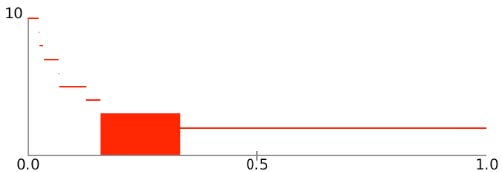
\includegraphics[width=\linewidth]{persistence-ui}
    \caption{Persistence curve showing the number of partitions as a function of persistence.}
    \label{fig:persistence-ui}
    \end{center}
\end{figure}


    \caption{Persistence curve showing the number of partitions as a function of persistence.}


\section{Regulus}
\label{sec:motivation}

While topological structures such as contour trees, merge trees and Morse-Smale complexes 
%are based on the function value at the critical points. It is important to note that while they do 
can capture features at multiple scales,
%and are often used to facilitate progressive simplifications, 
they nevertheless do not describe the simplification process, nor do they provide an overview of all the simplified topologies; rather, each instance describes, and is used to explore, only one simplified topology. Conceptually, simplification consist of creating a series of progressively coarse variation of one of these topological structures. In practice, only one model is created and then transformed to describe the required simplification level.
Visual exploration methods~\cite{Gerber10, maljovec16} are also designed to visualize one simplified topology at a time. Often, phenomena of interest appear at different scales in the data, and a single simplification threshold is insufficient for analysis.
The question of why should the user select a \textit{particular} simplification level was mostly left to the user's best estimation. 

In this work, we focus on the 'why' question in the context of using multi-dimensional Morse-Smale complexes  to study the relationships between input parameters and the output function. Rather than develop a method to find an optimal simplification threshold, our approach is to develop a visual representation of the whole persistence space that can help guide the user exploration. The new visualization, called Regulus Tree, is based on an interpretation of the simplification process in terms of nested partitions rather than cancellation on critical points. The expressiveness of the \RT comes to light when various attributes and measures are encoded on top of it. Another consideration of our design is to empower users to define their own attributes and measures and enable on the fly modification. The \RT enables,
% \begin{itemize}[itemsep=0pt]

    \noindent \textbf{Noise:} identify regions where noise is prominent
    
    \noindent  \textbf{Persistence level:} gain better understanding of the plateaus in terms of the size and stability of the partitions involves. Compare the statistical characteristics on the set of partitions for different persistence levels
    
    \noindent  \textbf{Adaptive simplification}: Select multiple persistence levels for individual features to adapt the simplification based on amount of relative rather than absolute noise, adapt to the local scale of features, and other measures of interest
    
    \noindent  \textbf{Local properties:} Compute and display local attributes of the function in different regions
    
    \noindent  \textbf{Relative measures:} Compare and contrast partitions from different locations in the function space as well as from different levels of details (persistence levels)
    
    \noindent  \textbf{Uniqueness:} Identify and study partitions that exhibit unique characteristics
    
    \noindent  \textbf{Clarity:} The \RT provide a hierarchical view of the persistence space in terms of nested partitions, which our collaborator scientists found much easier to grasp and comprehend as opposed to the technical description in terms of critical points cancellations. 
% \end{itemize}

In the following, we present the conceptual design, structure, and layout of the {\RT} as well as ways to simplify the tree itself. We describe several ways the \RT can be used for various tasks along with additional supporting views. We then introduce the notion of dynamic attributes and measures and show how they can provide unique insights and help guide the user exploration.

\section{The Regulus Tree}
\label{sec:regulus}

\subsection{The Regulus Partition Perspective}
A \MSC can viewed from two different perspectives. From a partition perspective, a \MSC describes a tessellation of the space into monotonic partitions.  From a formal perspective, it is described in terms of an intersection of ascending and descending manifolds, which generates cells including critical points, and arcs that connect them.  
% The simplification, on the other hand, is expressed only in terms of an ordered set of critical points cancellations, which maps well to the technical (based on critical points) perspective of Morse-Smale but not to the partitioning perspective. This dichotomy, in our experience, is the main reason for the confusion by some domain experts who are comfortable with the spatial partitioning perspective but find it difficult to comprehend the meaning and effects of canceling critical points. 
Cancellations, although involving only a pair of critical points,  may affect several partitions at once. This often poses a challenge for scientists in application domains using this approach, as the rules that govern the merging of spatial partitions are obfuscated by the simplified explanation.

Consider a single cancellation step, in which a pair of critical points is deleted as depicted in \autoref{fig:msc-overview}(c-e). From the partition perspective, the single simplification step consists of two merges of pairs of partitions. In general, and especially in multi-dimensional data, several merges can occur in each step, but each partition may participate in only one merger per step. Note that the actual simplification process stays the same and it is only our perspective that is changed. Furthermore, from the partition perspective, the partitions mergers form a \textit{nested} hierarchy and the full simplification process forms a binary tree. The leaf nodes of the tree represent the partitions of the initial More-Smale Complex (persistence level 0), while the root represents a single partition that encompasses the whole space. To construct a \RT we first create a full \MSC and then traverse the simplification list in order. For each simplification step we identify the pairs of merging partitions, create new nodes representing the merged partitions, and update the lists of internal and critical points associated with each new node (partition). Once we finish the traversal we descend down the new tree structure in a depth-first order and assign a sequential id to each node. We also reorder the data points to follow the order of the leaf nodes as described in \autoref{sec:tree} below. 

The notion of persistence as it applies to critical points does not directly apply to the nodes/partitions in the \RT. From the perspective of critical points, at each simplification step, one extremum is deleted while another one is retained, and no new extrema are added. The persistence of an extremum describes the value when the point is deleted.
In contrast, we regard the merger of two partitions as a new partition that describes a larger region of space with more data points and different properties and characteristics. The importance of this distinction arises when we fit regression models and evaluate various measures in each partition as described in \ref{sec:measures}. A partition is thus associated with \textit{two} persistence values describing its creation, original through Morse-Smale complex or through merger, and destruction, when it is merged. In the context of the Regulus Tree, we only need to save for each partition the persistence level it is created, as it is deleted at the persistence value its parent is created. The lifespan of a partition, i.e. the difference between the persistence levels of its parent and its own, provides a measure of the life-span of the partition.

% \begin{figure}[tb]
%     \begin{center}
%     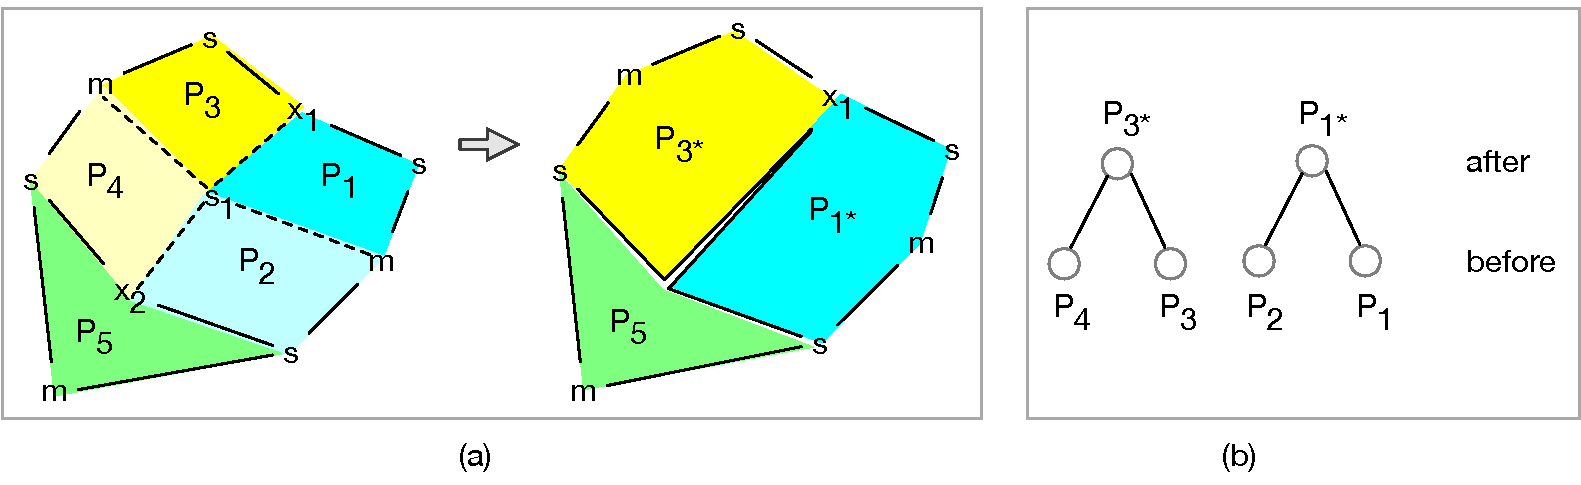
\includegraphics[width=\linewidth]{cancellation}
%     \caption{A simplification step over a 2-manifold: m, x, s represent local minima, maxima and saddles respectively. a) Merging x2 into x1 deletes x2, s1, and the internal edges. In addition, partition P2 merges into P1 and P4 into P3. b) The Regulus perspective represents the single step as two merges of pairs of partitions, forming two nested structures.}
%     \label{fig:cancellation}
%     \end{center}
% \end{figure}

\subsection{Regulus Tree Layout}
\label{sec:tree}
There are dozens of different ways to visualize a tree, yet conceptually all full tree layouts are based on either a top-down or a bottom-up ordering (\autoref{fig:tree-diagram}). The placement of a node is based on the distance of the node from the root (top-down) or a leaf (bottom-up) in terms of the number of parent-child edges. This is true whether the layout is vertical, horizontal, or radial. 
% In addition, tree layouts that employ edges between nodes are not space efficient in the sense that relatively little space is reserved for each node for depicting additional information about the node 

To the best of our knowledge, the \RT layout is new and unique. We describe the new layout in terms of modifying a bottom-up layout. First, we use the vertical axis to depict persistence level \autoref{fig:tree-diagram}c). We then represent a tree node by a rectangle and position it vertically such that its bottom edge is aligned with the persistence level in which it is created. Because the leaves of the tree represent the base partitions, i.e. the partitions of the full \MSC before any simplification, they must, by definition, have a persistence level of 0 and therefore form a single row of rectangles whose bottoms are all aligned. 

When two partitions are merged, the new partition (the parent) must have a persistence level greater than that of its children and thus will be positioned vertically higher than its children. In the horizontal direction, we use the width of the rectangles to encode the number of data points and convey a measure of size. Note that if the data points were sampled uniformly, then the number of points in a partition is roughly proportional to its volume. Since, by definition, a parent contains all the points of its direct children, then the width of the parent is equal to the sum of the widths of its children. Therefore, we can position all the children of a parent sequentially in the horizontal direction without causing overlaps (\autoref{fig:tree-diagram}d). Finally, we extend the top of each node to the base of its parent. The height of a node therefore encodes its lifespan since the base of the parent represents the persistence level the parent is created and the level in which the children are deleted. We note that the vertical axis of the \RT represents persistence and not function value as used in other techniques, such as the contour and merge trees, or the persistence diagram.

\begin{figure}[tb]
    \begin{center}
     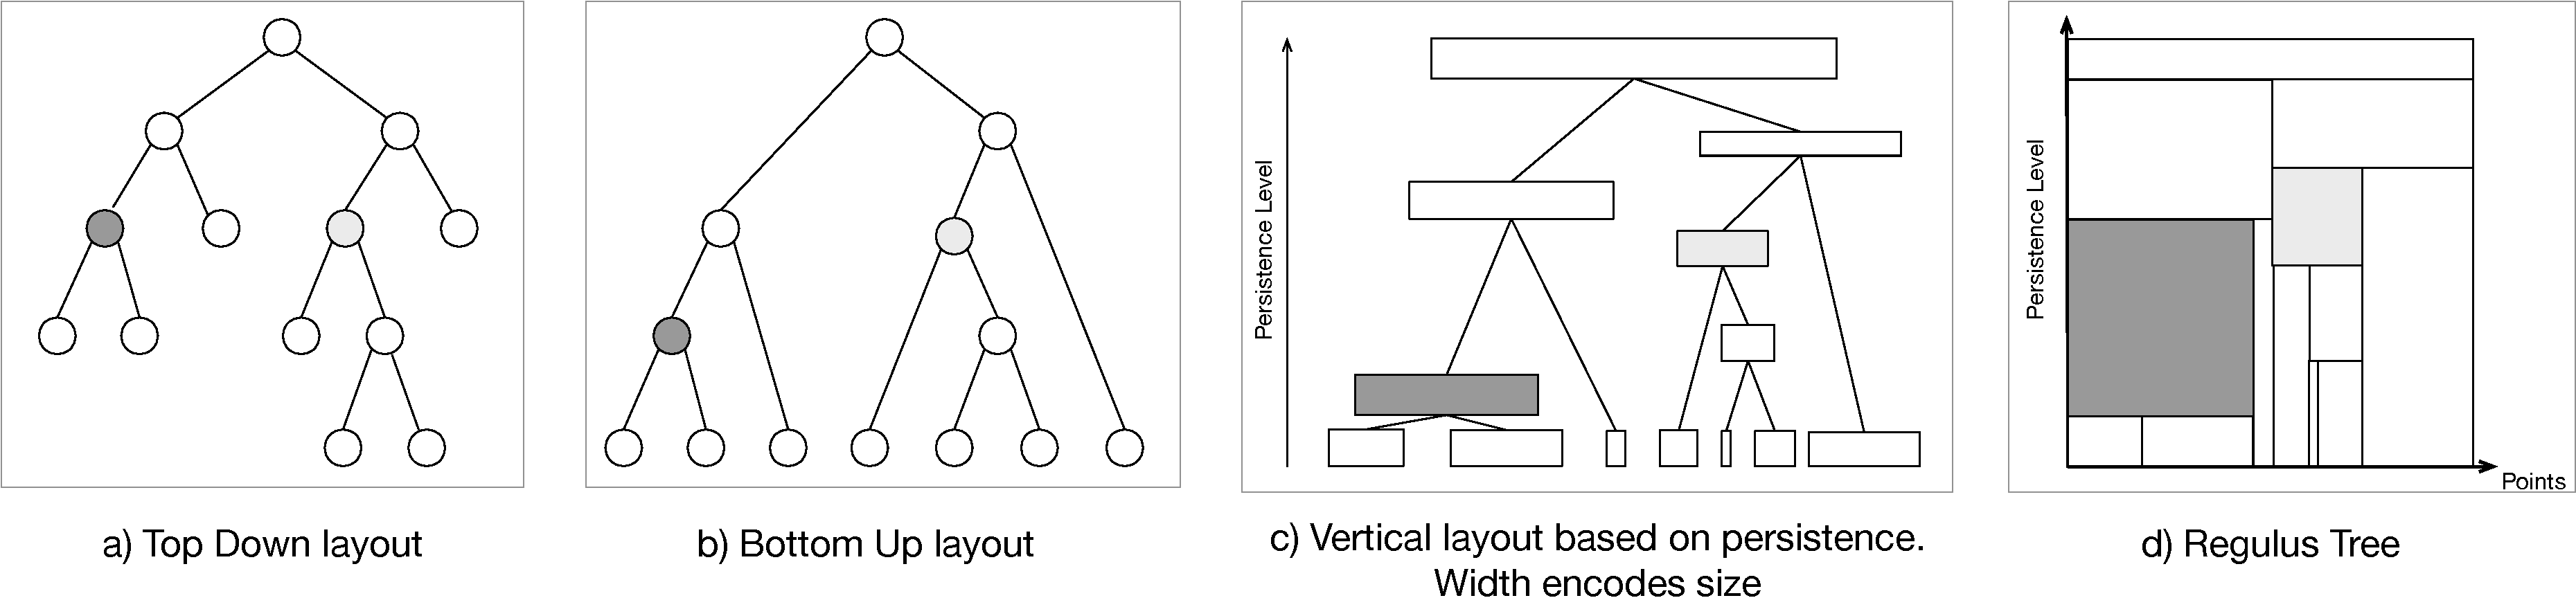
\includegraphics[width=\linewidth]{tree-diagram-1}
    \caption{Typical tree layouts position nodes based on their distance from the top (a) or bottom (b). We use vertical position to encode persistence and width to encode size (c). \RT (d): node height extends to parent to encode lifespan; horizontal layout based on enumeration of the points. Two of the nodes are shaded to illustrate the correspondence between the trees.}
    \label{fig:tree-diagram}
    \end{center}
\end{figure}

We can take advantage of the horizontal layout by enumerating all the data points based on the base partitions they are part of (the enumeration within a partition is not important). Using this approach, we need only two numbers per partition to indicate the range of data points that are contained in that partition. Since the parent partition contains all the data points of its children and the children are positioned sequentially, the partition's data points can also be specified via a range using two numbers. Effectively, we decoupled the data points from the hierarchical structure of the partitions and kept the memory size at $O(n + p)$, where $n$ is the number of data points and $p$ is the number of partitions in the tree.

It is important to note that the above description is correct only with respect to non-critical points, which are shared between partitions. To address this, we initially assign each critical point to one of the base partitions adjacent to it. We then maintain for each partition a short list of all the critical points it's associated with but are not part of its own range of points. In the tree layout, we use the width of a node to encode only the number of points its children contain. This ensures that the parent has the correct visual width to contain all of its children. The exact number of points associated with a partition is provided in a tooltip. This does not pose any problems as the number of extra critical points is minimal. 

\autoref{fig:regulus-tree} shows a \RT associated with a $2d$ scalar function, which we sampled at 2000 points and added small white noise. The horizontal axis represents enumeration of all 2000 points, while the vertical axis represents the relative persistence level in the range of 0 to 1. For illustration purposes we use color to encode the lifespan of each node, i.e the difference between the persistence value of the parent and the persistence value of the node. 

The \RT is \textit{not} a TreeMap despite the superficial similarity. A TreeMap depicts the leaves of a tree using a 2D layout that takes into consideration the tree hierarchy, and the two axes do not have individual meaning. A few variations do incorporate some information about the parents, but because the emphasis is on the leaves, the parents are depicted differently and are mainly used to convey structure. In contrast, the \RT represents the whole tree structure, the two axes have precise and different meaning and for the most part the leaves are the least important features.

\begin{figure}[tb]
    \begin{center}
    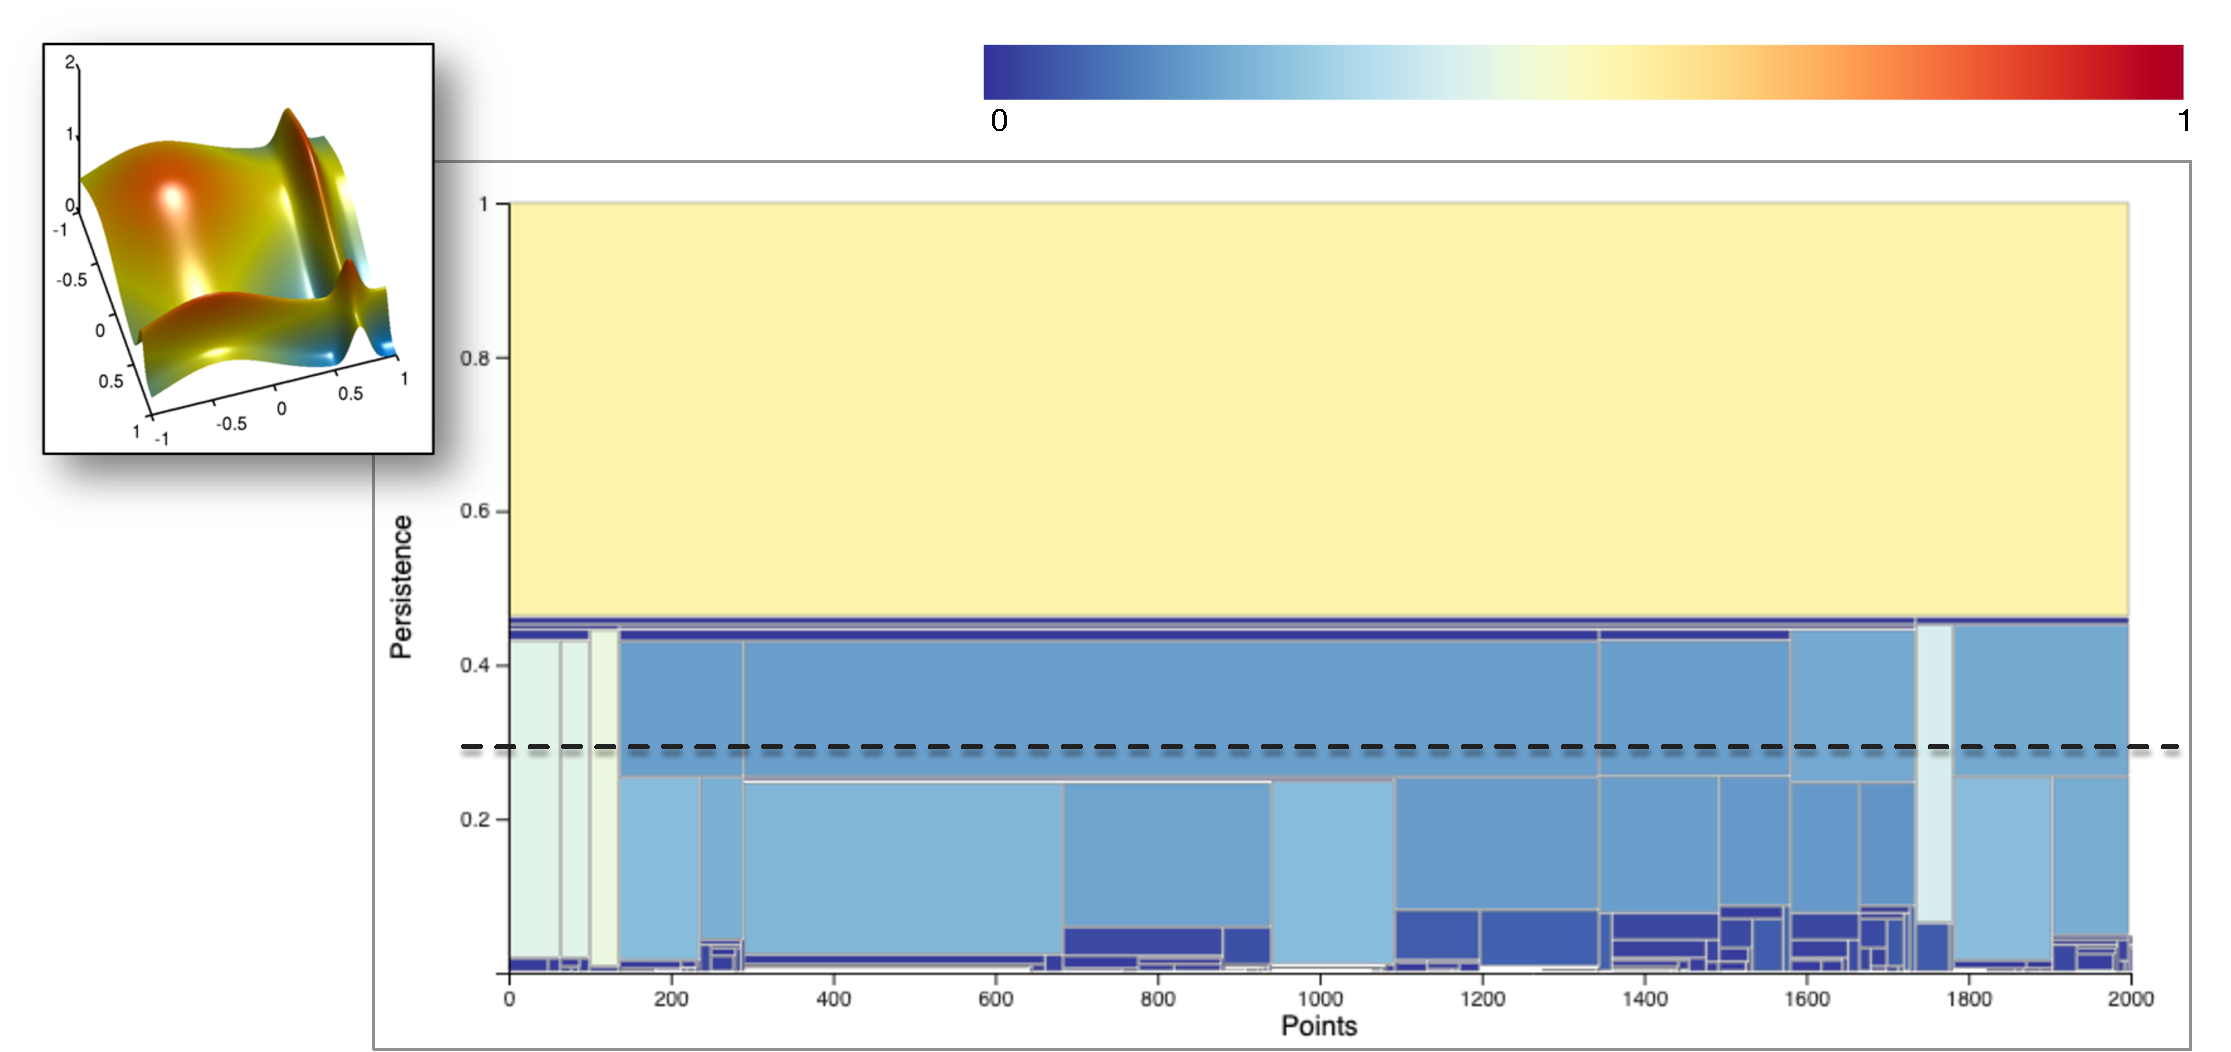
\includegraphics[width=\linewidth]{example}
    \caption{A 2D scalar function and a corresponding \RT. For illustration purpose, color encodes the lifespan of a partition using the blue-yellow-red colormap shown at the top. Selecting persistence level of 0.3 amount to selecting the nodes that intersect the dashed line.}
    \label{fig:regulus-tree}
    \end{center}
\end{figure}

\subsection{Simplifying the Tree}
\label{sec:filtering}
Despite its compactness, the \RT can become quite large for large datasets with complex topology. In addition to pan and zoom, we can also visually simplify the tree without changing the layout by hiding nodes based on some filtering criteria. In both cases only the visualization of the tree is modified but not the tree itself. More often than not, though, we want to simplify the tree itself.

Persistence is often used to help separate between noise and real features by removing features with low persistence level, which amounts to pruning the tree at a certain  threshold. From the technical perspective, persistence provides some measure of the dominance and stability of a critical point, suggesting which features should be preserved. The partition perspective of the \RT offers a different way to think of persistence. Consider the \RT depicted in \autoref{fig:reduce}b and the two narrow green and purple partitions, both of which have a relatively short lifespan but may actually represent a merger of two prominent features. The higher the node is located along the vertical axes, the higher the persistence levels of the two features being merged and the deeper the valley between the two mountains is (or the taller the ridge between two valleys is). 

From the perspective of the Regulus Tree, such partitions are unstable and can be regarded as a relative noise within their local neighborhood. In terms of creating a simplified description of the topology, removing these partitions is akin to depicting a mountain range by only one or two mountains. We  extend this notion of simplifying the topology by simplifying the \RT to also include removing small partitions (thin partitions with few points), partitions with points with values outside a range of interest, and in general filtering the function the user may wish to apply.

While removing small noise amount to pruning the tree, filtering specific nodes does not amount to removing their children. Instead we attach the children to their grandparent  (\autoref{fig:reduce}a), which means that in general a \RT is not a binary tree. We compute a full tree simplification by traversing the tree depth-first and considering one node at a time. If many nodes are removed the new tree may end up with tall and skinny nodes. This is especially the case if we insist on keeping base partitions even if the original lifespan is too small. Our approach is to remove such base partitions and allow the tree to have a jagged edge at the bottom (\autoref{fig:transition}). 
 
We do need to ensure that the new tree represents a valid simplification of the topology. Since a node/partition is the sum of its children, it contains all of their points and thus the grandparent must by definition already contain the points of its new direct children. Another issue to consider is the lifespan of the remaining partitions. We defined the lifespan as the difference between the persistence levels of the parent and the partition. For this reason, we do not store the lifespan of a partition in the partition record; rather, we compute it on the fly based on the parent-child relationship of the node pointing to it. The lifespan of a partition is therefore relative to the tree pointing to it and a partition may have different vertical height (lifespan) after the simplification/transformation of the tree. 

In general, we do not modify the original tree; rather, we create a new tree hierarchy that refers to a shared collection of partitions. In this sense, each tree is a view over the collection of partitions, similar to creating a sub-array as a view of the full array. 
% The separation between the tree structure and the collection of partitions allows us to create multiple trees all pointing to the same set of partitions, although each tree may refer to only some of the partitions. This in turn allow us to visualize multiple trees side by side, representing variation of nested hierarchies, a kind of collection of meta-simplifications of the topology. 

\begin{figure}[tb]
    \begin{center}
     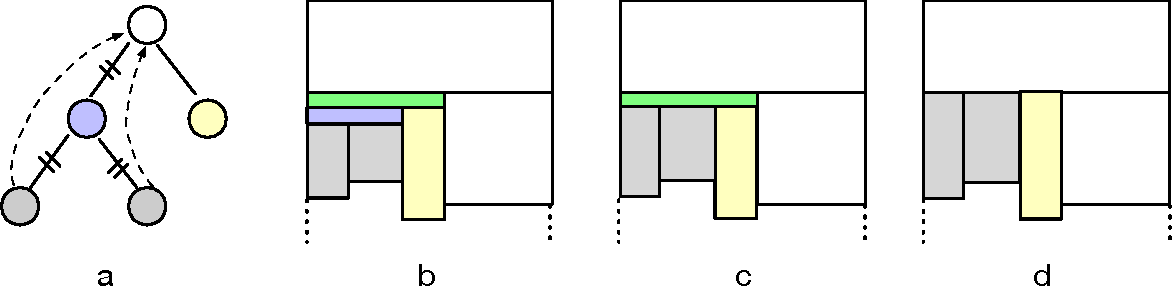
\includegraphics[width=\linewidth]{reduce-2}
    \caption{Simplifying a Regulus Tree by removing intermediate nodes. 
    % The parent node represents multiple half simplification steps (recall that one simplification step leads to multiple partitions merges).
    }
    \label{fig:reduce}
    \end{center}
\end{figure}


\subsection{Exploration and Simplifications Strategies}
\label{sec:simplification}

In addition to providing a concise global overview, the structure of the \RT can be used to help guide the exploration and determine where to simplify, 
\begin{itemize}[label={}, leftmargin=0pt, noitemsep]
    \item  \textit{Global simplification}: In the context of the Regulus Tree, a persistence value maps to a single horizontal line as shown by the red dashed line in \autoref{fig:strategies}a. Since we do not compute level sets, it doesn't matter where the line intersects a partition, only that it does.  While the persistence graph only indicates the number of active critical points for the given persistence value, the \RT provides insights about the size (width) and stability (height) of the partitions. The tree structure may, for example, reveal  that a section of the persistence graph that is not a plateau is actually composed mostly of stable partitions throughout the domain except for instabilities in a small part of the domain or maybe in a number of small partitions that are likely not significant.

    \item  \textit{Adaptive simplification}: Consider a height function depicting the geographic elevation of a valley in a mountainous area. Perturbations that might not be important in the rugged mountains may have significant importance in the flat valley area. We can apply the notion of local simplification in the context of the \RT by selecting a step like line, such a the red line in \autoref{fig:strategies}b. We do not alter the meaning of the simplifications. We only select a subset of the original simplifications. No new partitions are introduced.
    
    The adaptive simplification is easy to understand in the context of the \RT but computing the boundary or interpolating a continuous function across the selected partitions might not be a trivial task as the boundary will include T-junctions. This is not an issue in the context of this work as we focus on understanding the general structure of the underlying function and identify interesting regions.
    
    \item  \textit{Discrete selection}: Supporting a selection based on single persistence value is simple as it requires moving a single horizontal line up and down. The local simplification is more complex and would require interactive construction of a line with potentially multiple steps (adding and removing steps, adjusting step vertical and horizontal positions). A simpler approach is to allows the user to directly select (e.g. click on) the partitions the step line should pass through \autoref{fig:strategies}b.
    
    \item  \textit{Non-continuous selection}: For the purpose of identifying and exploring interesting partitions, it is sufficient to select only partitions of interest (\autoref{fig:strategies}c) to quickly compare and contrast the properties of partitions at different persistence levels. This is by far the most often used selection method we employ in our workflows.
    
    \item \textit{Non-consistent simplification}: We can generalize the non-continuous selection by selecting partitions that overlap horizontally, that is a partition and its descendent (\autoref{fig:strategies}d). There are two reasons for using  non-consistence simplification. One is to simply compare the properties of a partition with its parent to determine if the parent provides sufficient details. The process can be repeated up and down the tree hierarchy if a more fine tune simplification of the whole \MSC is required. The second reason has to do with efficient representation. Consider a quadtree partitioning of a relatively smooth function except for one small area as shown in \autoref{fig:strategies}e. This space decomposition is often critical in many applications, despite the fact that 12 of the 13 partitions are very similar. On the other hand, when studying the structure of the underlying function, a more efficient representation might consist of only two nested regions as shown in \autoref{fig:strategies}f, which provides both a global view and local details.
\end{itemize}

\begin{figure}[tb]
    \begin{center}
    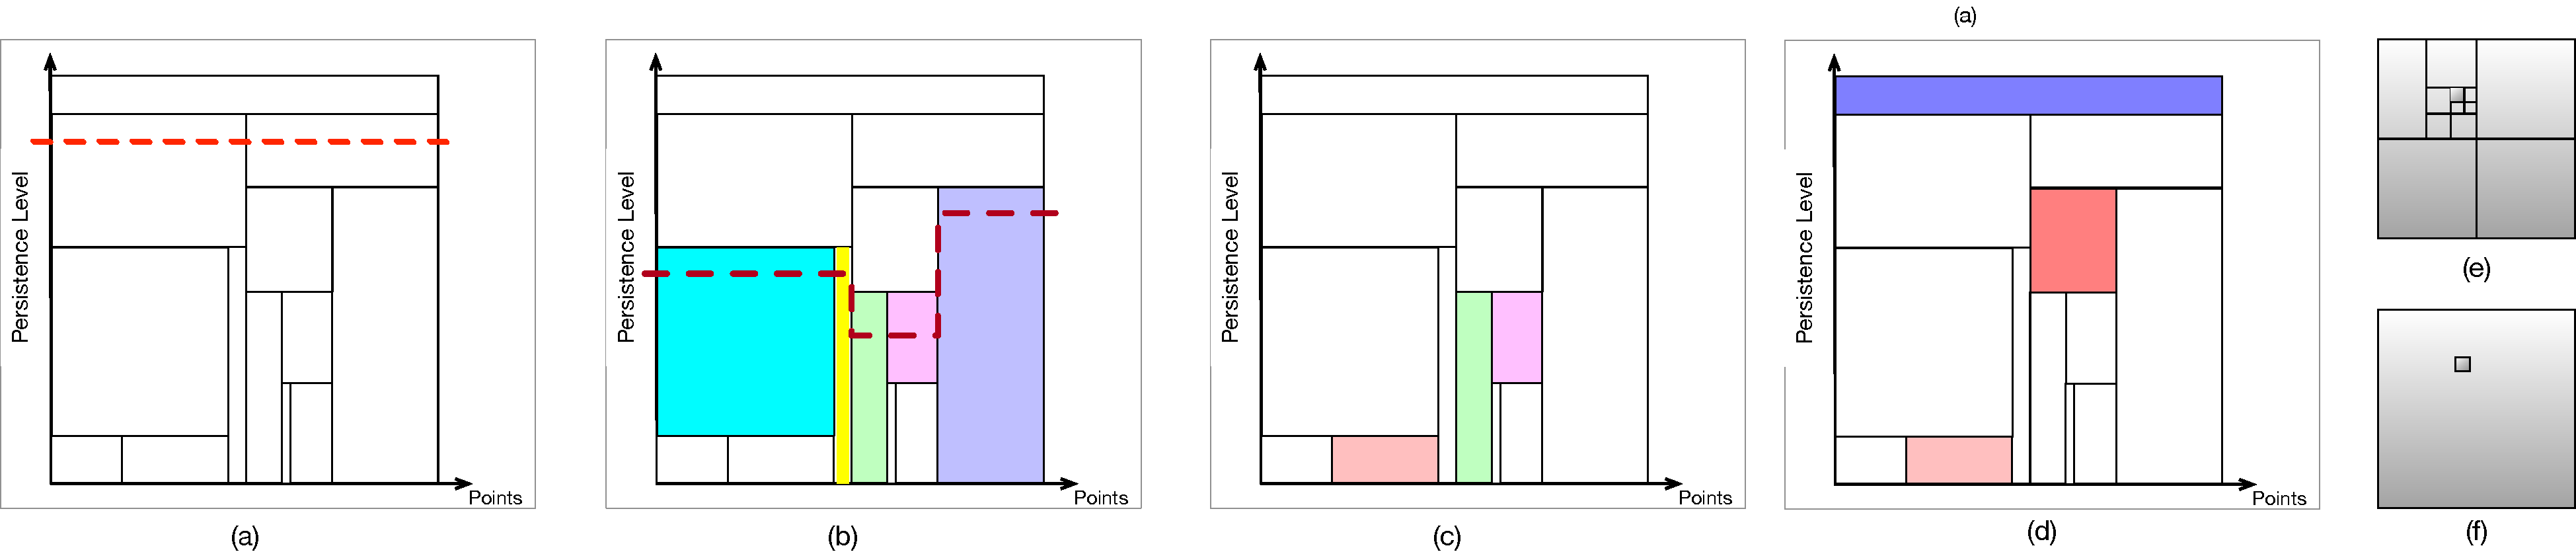
\includegraphics[width=\linewidth]{strategies-4}
    \caption{Exploration strategies. a) global simplification b) adaptive simplification c) non-continuous selection d) non-consistent simplification. e-f) The rational for non-consistent simplification (see text)}
    \label{fig:strategies}
    \end{center}
\end{figure}

 

\vspace{-.1in}
\section{Views}
The \RT provides an overview of the hierarchical persistence space, but it does not provide any direct view of the data points, nor does it provide direct relations between the partitions. The variable size of the nodes also makes it harder to encode multiple values for each node. In the following, we provide a short descriptions of two additional views we employ. 

\subsection{Details View}
% The details view provides additional insights about a selected partition in terms of projections of its points, the inverse regression curves, and the coefficients of the linear regression curves.

The details view (\autoref{fig:fitness}) depicts a set of scatterplots for a set of selected partitions where each row represents one partition and each column represents one input dimension. Each scatterplot depicts the points in the partition, where the y-axis represents the scalar function value and the x-axis represents the specific input dimension. The same y-axis range is used for all the plots across all the rows and columns. The x-axis range depends on the dimension (column) but is the same across all rows. The points are colored using the same blue-yellow-red color map and initially encode the value of the output function similar to the y-axis. Some datasets include multiple output values, only one of which is used to create the base Morse-Smale complex. The color can be used to encode any of the output variables. The partition id and the number of points in the partition (in parenthesis) are shown in the left most column. 

Each plot also depicts a projection of the inverse regression curve for that partition. The semi-transparent area on both sides of the curve corresponds to one standard deviation for the corresponding input dimension. 
% Together, the inverse regression curves and the standard deviation provide a concise summary of the local behaviour of the function. 
% We also use the inverse curves as skeleton representations for selecting additional points to sample the underlying scalar function, but this work is beyond the scope of this paper. 

We encode the coefficients of the linear regression models as horizontal bars under the plots. The bar in the left most column encode the intercept of the model. Green/red indicate a positive/negative coefficient respectively. The coefficients are normalized either with respect to current model or with respect to all the selected models. 

\subsection{Graph View}
The graph view depicts a 2D projection of selected partitions (\autoref{fig:graph}). Each partition is represented by an edge between its minimum and maximum critical points. There are many dimensional reduction methods, each with its own merits. One of a recurring complaints we receive from our collaborators is that the abstract nature of the projections often makes it very hard to comprehend and make use of. We designed the graph view to both simplify the projection and to allow the scientists to interactively explore the projections in ways that are meaningful to them. A point in multi-dimensional space is a linear combination of unit vectors each pointing along one dimension. In the Graph view we depict it as a linear combination of vectors in the 2d plane. The user can scale and rotate the vector to change its relative contributions as well as focus on specific dimensions by removing some of the vectors.

The graph view can also project the points in the selected partitions. The points colors encode the same information as in the Details view. When a partition is highlighted, the points not in that partition are rendered as small gray points. A partition is highlighted when the user hovers over the partition edge in the graph view, hover over the partition in the \RT view, or hover over the partition row in the details view. Finally, the partition's edges can be rendered by projecting their inverse curves. Although these curves are not guaranteed to end up in the appropriate critical points, they often provide a good insight about the structure of the partition.

\autoref{fig:graph} depicts three projections of the test dataset. The projection on the right demonstrates that manipulating the vectors can provide meaningful projections, in this case conveying a pseudo 3D perspective. The ability to individually manipulate each dimension proved valuable in exploring the contribution of individual and groups of dimensions. For example, by combining, subtracting and contrasting the contributions of several dimensions (same, opposite or perpendicular directions), as shown in \autoref{fig:combustion-projections}. 



\vspace{-.05in}
\section{Coloring the Tree}
\label{sec:analysis}
The structure of the \RT provides initial insights about the \MSC that describe the underlying scalar function in terms of the distribution, size, and persistence of the partitions. The expressiveness of the \RT becomes apparent when we encode additional information about the underlying scalar function. In particular, we fit linear models to the data points in each partition and compute various measures that provide insights about the local behaviour of the underlying scalar function within a partition, as well as comparison between different partitions. 

% \subsection{Workflow}
% Examine the tree looking for: 
% \begin{itemize}
%     \item local simplification. how far up the tree can we go simplify the \MSC
%     \item look for partitions with unique behaviour (linear models)
%     \item simplify the tree itself
% \end{itemize}

\subsection{Attributes and Measures}



Each partition has several inherent attributes, such as the number of samples it contains and the persistence levels where it's created. Additional attributes, such as the min and max values of the function within the partition can be precomputed and saved. Precomputing attributes introduce several challenges. First, while some attributes are fast and cheap to compute and store, others, such as inverse regression curves, require substantial time and space, especially if precomputed for all the partitions in a large tree. Second, many partitions may not be of interest for various reasons such as if they were created due to noise in the data, have too few data points, or have a very short lifespan. Since we often filter out or hide these partitions, precomputing their attributes would be a waste of resources. Third, some attributes describe relative measures between partitions, such as between parent and child, that depends on the particular tree. For example, the lifetime of a partition is the difference between the persistence values for the creation on its parent and itself. Fourth, some attributes, such as the bandwidth used in computing reverse regression curves, depend on parameters the user may change during the exploration, and which will require to recompute them on the fly. Finally, we want to empower users to define and modify their own attributes on the fly.

Our solution is to add the notion of a measure, that is, an attribute that is defined by providing a function to compute it rather than providing its value. A measure will be lazily evaluated for a node and the value will be cached in memory, though the user can save the cached values and the measure function to a file and reloaded next time. The use of measure functions, lazy evaluation, and caching are opaque to the rest of the system, which uses them as regular maps of node id to value. Using this approach allows us to define many attributes without the computational costs, as well as add and modify attributes and measures on the fly. When visualizing a Regulus Tree, we only need to ensure the selected measure was evaluated for the visible nodes. 

Often, several measure functions use similar computations, such as fitting a regression model for a given partition and then computing some derived values. We address this by defining the shared computation as a separate measure, which the other measure functions then retrieve rather than call directly. 
% \autoref{fig:attr-def} shows a simple definition of the lifespan measure. The tree parameter enable the measure to retrieve other attributes/measures of the node.

% \begin{lstlisting}[language=Python, float=tb, label=fig:attr-def, caption=Measure definition, aboveskip=\tinyskipamount]
% def lifespan(tree, node):
%     return node.parent.persistence -
%           node.persistence
           
% tree.add_attr(lifespan) # add measure definition to a tree
% \end{lstlisting}

\subsection{Regression Models}
\label{sec:models}
To study the function behaviour, we employ regression analysis to fit local linear models in the various partitions. As a first step we standardize the full dataset by removing the mean and scaling to unit variance.  We fit a model to each partition independently of any neighboring partitions. The main reason is that a partition can be explored in a variety of settings each leading to different sets of neighboring partitions or even none at all (\autoref{sec:simplification}). We do not want the model of a partition to change during the exploration based on indirect actions. 

A linear model is expressed in terms of a set of coefficient, $\beta_i$ such as that $ \tilde{y} = \sum_i^d x_i \beta_i + \beta_0$,
where $\tilde{y}$ is the predicted value and $\beta_0$ is the intercept. A least square regression model is obtained by minimizing the residual sum of squares between the observed and predicted values, 
\[ \min_\beta\| X\beta - Y \|_2^2 \]
To address the potential problem of multicollinearity in the linear regression, which is common in models with large number of parameters, we use Tikhonov regularization, also known as Ridge regression, which constrains the solution by imposing a penalty on the magnitude of the coefficients,
\[ \min_\beta\| X\beta - Y \|_2^2 + \lambda\| \beta \|_2^2 \]
where large $\lambda$ leads to smaller coefficients and a more robust solution to collinearity.

Our attributes and measures approach allows us to accommodate different regression models and freely switch between them during an investigation. We first define a set of model computational functions and then assign one as the current model measure, see \autoref{code:models}. Measures that depend on the regression model in a partition can fetch the 'model' attribute as shown in \autoref{code:fitness}. The model can be replaced at run-time, which in turn invalidates all the models that were already computed, as well as all other measures that depend on it.  

\begin{lstlisting}[language=Python,caption=Using different regression models., 
    float=hbt, label=code:models]
def linear_model(tree, node):
    return LinearRegresssion().fit(node.x, node.y)
def ridge_model(tree, node):
    return Ridge().fit(node.x, node.y)
tree.add_attr(ridge_model, name='model')
\end{lstlisting}

Higher order regression models can also be used although they are more complex and in some sense defeat the purpose because they are not monotonic and it is difficult to interpret their coefficients. High-order model also suffers from the curse of dimensionality; a linear model requires d+1 parameters to describe an d-dimensional data but a quadratic model requires $O(d^2)$ parameters.



\vspace{-.05in}
\subsection{Measures}
\label{sec:measures}

Basic measures we often use include the lifespan, minimum and maximum value, and normalize size. We also define measures to assign a unique id (encoded as different colors) to minima and maxima critical points that are shared between partitions. A shared minima/maxima measure shows the tree from a perspective of merges of minimum/maximum critical points, which in some sense is similar to a merge tree.


\begin{lstlisting}[language=Python, caption=Fitness score (not suitable for derived trees), float=b, label=code:fitness]
def fitness(tree, node):
    model = tree['model'][node]
    return model.score(node.x, node.y)
def parent_fitness(tree, node):
    parent_model = tree['model'][node.parent]
    return parent_model.score(node.x, node.y)  
def child_fitness(tree, node):
    model = tree['model'][node]
    return model.score(node.parent.x, node.parent.y)
\end{lstlisting}

\subsubsection{Fitness}
\label{sec:fitness}
Given a linear regression model for a partition, the first question is how well the linear model actually fits the data. The \MSC guarantees that the data is monotonic within a partition at persistence level 0 but it does not imply linearity. Level 0 partitions that do not have a good linear model fit imply the function was undersampled. At higher persistence levels, multiple partitions with good but different linear models might merge into a single partition with a bad fit (e.g. partitions 0 and 45 in \autoref{fig:fitness}). Identifying such instances can be used to determine to locally choose a persistence value lower than the merged partition. 

We evaluate the fitness of a regression model using \textit{coefficient of determination}:
$R^2 = 1 - \frac{\sum (y - \tilde{y})^2}{\sum (y - \hat{y})^2} $,
where $\tilde{y}$ is the predicted value and $\hat{y}$ is the mean value. The score value range between 1.0 (perfect fit) to $-\infty$. A model that always predicts the expected value of $y$ disregarding the input would have a score of 0. 

\textbf{Example:}
\autoref{fig:fitness} (middle right) shows the \RT of the 2D function from \autoref{fig:regulus-tree}. In this case, we encode the fitness score of the linear model in each partition as color after we clamped it to the range 0 (blue) to 1 (red). The details view, \autoref{fig:fitness} left, shows projections of data points in several selected partitions. 

In general, the higher a partition is positioned alone the vertical axis the lower the fitness score will be (less red) as each merger add more points, which by definition can only reduce the fitness. The numerical value of the current attribute is displayed via a tooltip along with additional information. Partitions 21 and 34 have very good models (0.94 and 0.96 respectively) although they are very different from each other with respect to the $x1$ dimension. This difference is reflected in their parent, partition 20, which has a lower fitness score (0.77) due to the nonlinearity the merge introduced in the $x1$ dimension. 

The shallow hill (top left in the 3d view) contains over half the data points and is captured by partition 45 as a merge of four partitions with very good but very different linear models, leading to a fitness score of only (0.42). Close examination (zooming) confirms that two of the partitions merge first, followed by a merge with the third and fourth. The two intermediate partitions are not stable and have a very short lifespan. Finally, the root of the tree, partition id 0, consists of the entire domain (2000 sample points), and represent the case where we simplify the \MSC all the way down to a single partition. As can be expected, the fitness score is only 0.38 since there is no good global linear model for the data. 


\begin{figure}[bt]
    \begin{center}
     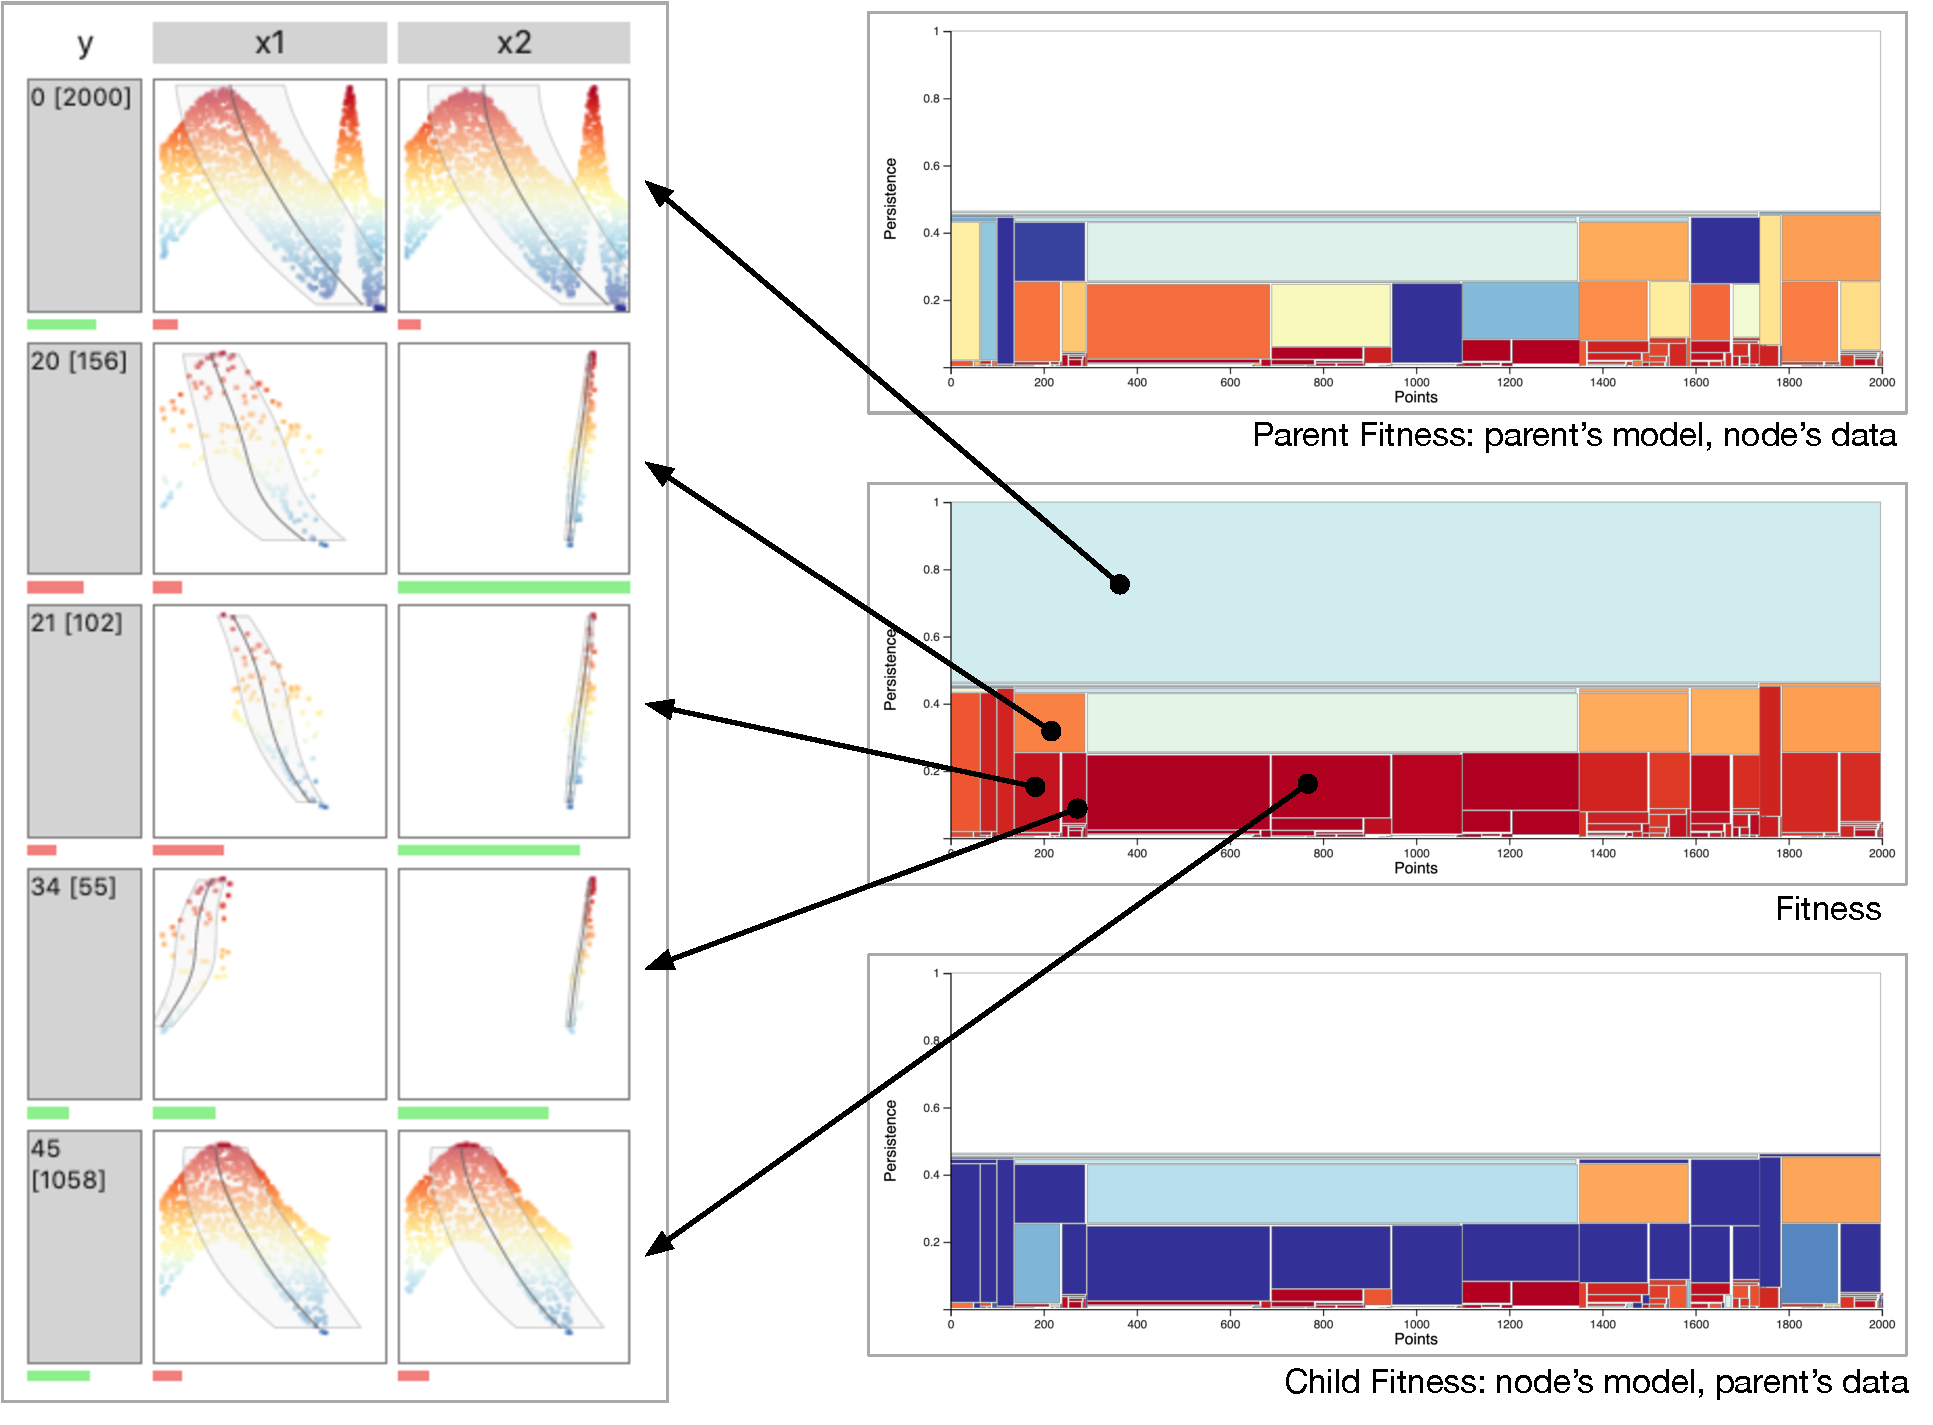
\includegraphics[width=\linewidth]{details-5}
    \caption{Left: details view showing points in selected partitions. Right: Three views of the Regulus Tree, each showing separate fitness measure (blue = 0, red = 1)}
    \label{fig:fitness}
    \end{center}
\end{figure}

\textbf{Parent and Child Fitness}
Partitions 20, 21 and 34 in the above example, highlight the case where a merger of two partitions, both with very good linear models, can lead to a partition with a much worse fitness score. In this case, we should avoid simplifying further at least locally. The different situation can arise where the parent model is very similar one of the children but not the other one. \autoref{fig:fitness-issue}
depict a potential merger between two partitions for a 1d scalar function, where both the children and the parent have good linear models. If we rely only on the fitness score of the parent, we may conclude that the parent represents a good simplification choice, a decision we may not take if we examine at the actual data. This scenario can occur, for example, when one partition contains a lot more data points then the second partition. In some applications, this can be addressed by giving different weights to the points in the two partition. In the context of this work, we specifically want to identify and flag situations like this as they are likely pointing region where the scalar function have unique characteristics. Furthermore, we would like to be able to detect these cases directly in the \RT without the need to examine the data points.
\begin{figure}[b]
    \begin{center}
     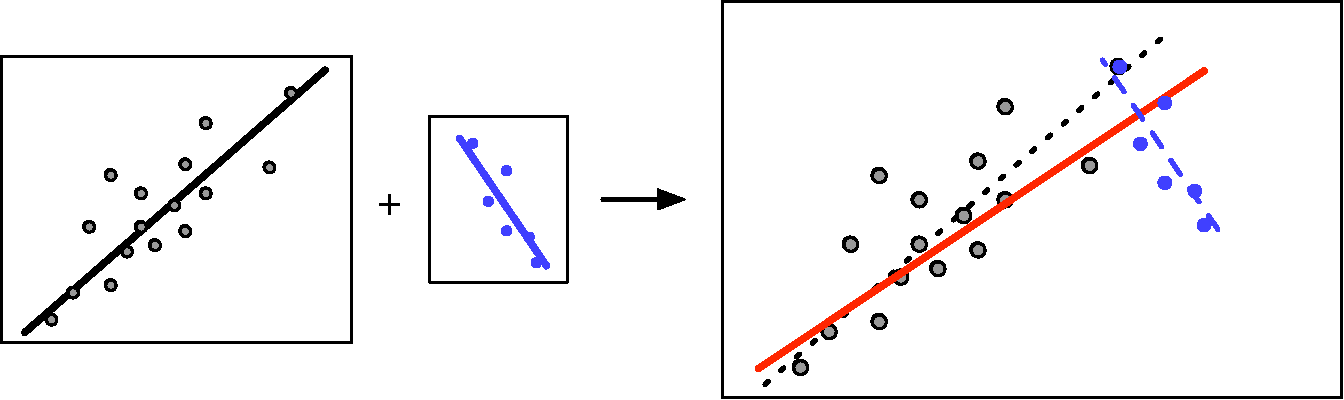
\includegraphics[width=.8\linewidth]{fitness-issue-1}
    \caption{A merge of two partitions with good but different models can lead to a partition with a model that is similar to only one of them.}
    \label{fig:fitness-issue}
    \end{center}
\end{figure}

To address this issue we introduce two \textit{relative} fitness measures as shown in \autoref{code:fitness}. The \textit{Parent Fitness} is the fitness score of the parent's model with respect to the partition data. Conversely, the \textit{Child Fitness} is the fitness score of the partition model with respect the parent's data. Referring back to \autoref{fig:fitness}, the parent fitness is shown in the top right tree and the child fitness in the bottom right tree. The parent fitness indicates that the model of partition 20 moderately fits the data in partitions 21 and 34 (0.79 and 0.65 respectively). The child fitness scores clearly show that the models for partitions 21 and 34 do not fit well with their parent's data (0.2, -1.8 respectively), strongly implying that this simplification step should not be used.



\textbf{Example part II:}
Using the combination of fitness and child fitness scores, we can see that a persistence level of 0.2 provides a very good simplification value. \autoref{fig:graph} shows a top down projection of the full \MSC and both top down and side view projections of the simplified \MSC.  We designed our visual exploration environment specifically to cater to this kind of workflow where multiple measures need to be considered at the same time. The user can visualize multiple \RT instances, each encoding different measures, or simply define a new measure that returns a value based on evaluation of the the fitness, child fitness, and parent fitness in the partition.

\begin{figure}[bt]
    \begin{center}
     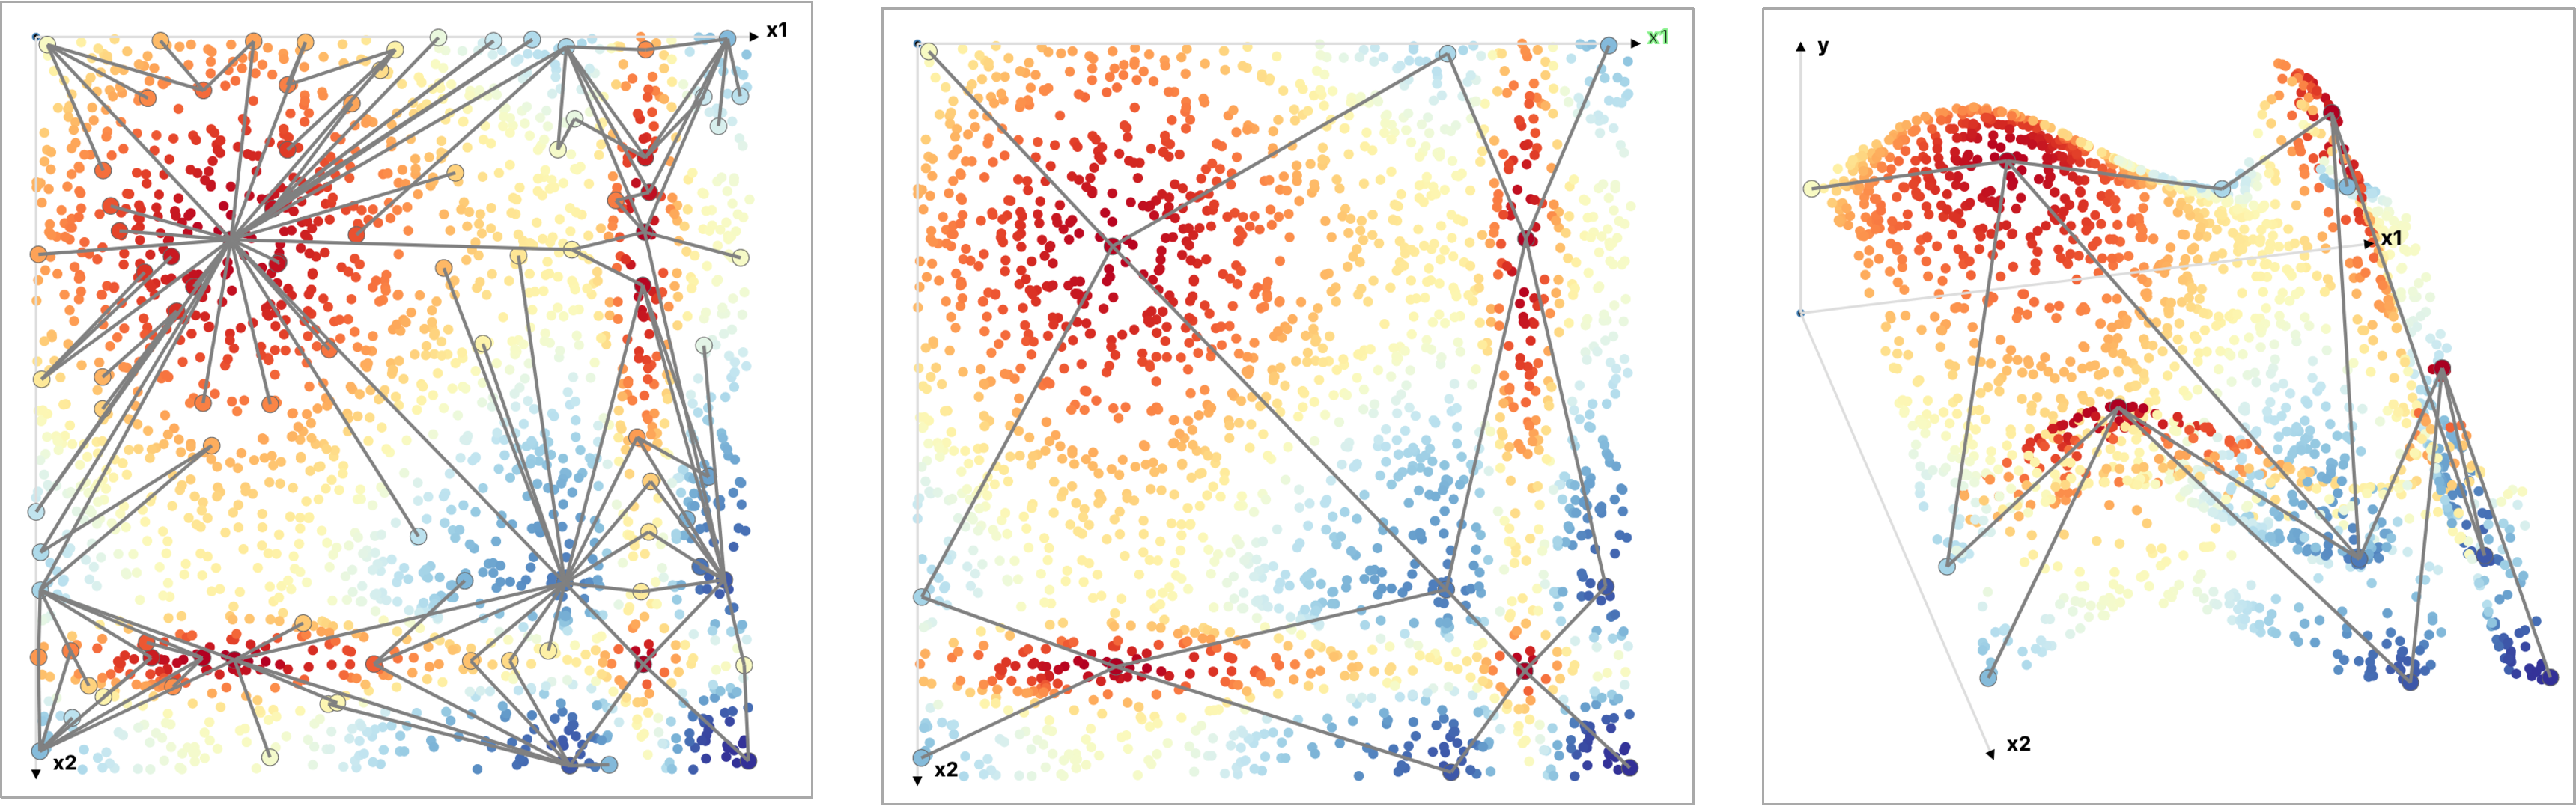
\includegraphics[width=\linewidth]{gauss-graph2}
    \caption{Left: Graph view of the full \MSC and the data points as viewed from above. Middle: Simplification for persistence level = 0.2 Right: Adding the y-axis and slightly rotating the x1- and x2 axis generates a pseudo 3D projection.}
    \label{fig:graph}
    \end{center}
    \vspace{-0.15in}
\end{figure}

\textbf{Reference Model Fitness:}
The parent and child fitness measures play an important role in our workflow despite being limited to only the local neighborhood of a node. As a side note, we do not define a fitness measure between siblings because in the case of derived trees (see \autoref{sec:filtering} a partition can have more than two children. The advantage of the local nature of the parent and child fitness measures is that we can depict each measure over all the nodes in the tree at once. There are cases, however, where we want to compare and contrast models for more distanced ancestors and even between partitions in different parts of the tree (recall that the tree is organized with respect to the list of merges generated using persistence homology not based on local geometry). Depicting many independent global comparisons at once is not possible. Instead, we define a \textit{reference model fitness} measure that applies a reference model to the data in each partition. When the user hovers over the tree we set the reference model to the model of the node under the mouse and reset the cache to cause the values to be recomputed.

% \begin{lstlisting}[language=Python, caption=Fitness score, float=htb, label=code:reference-fitness]
% def reference_fitness(tree, node):
%     reference_model = tree['reference_model']
%     return reference_model.score(node.x, node.y)  
% \end{lstlisting}

\textbf{Dimension Fitness:}
Regression methods fit linear regression models by minimizing cost functions that take into consideration all the dimensions of the data. In that sense the cost (error) is spread over all the dimensions. Within the context of this work, we are trying to identify unique partitions, which means we aim to find maximum discrepancies between partitions and in particular with respect to individual dimensions.

Our \textit{dimension fitness} approach is to compute a vector of regression models for each partition, one per dimension, instead of a single model. Scoring in this case means applying each model in the vector to the data, resulting in a vector of scores instead of one value. Given two partitions, we apply and score the model vector of one partition to both data sets and finally compute the cosine similarity between the two score vectors (\autoref{code:dim-fitness}).

\begin{lstlisting}[language=Python, caption=Dimension Fitness, float=hbt, label=code:dim-fitness]
def relative_dim(tree, models, data):
    return [models[i].score(data.x[i], data.y) 
            for i in range(len(models)]
def child_dim_fitness(tree, node):
    models = tree['dim_models'][node]
    return cosine_similarity(
        tree['relative_dim'][models, node],
        tree['relative_dim'][models, node.parent])
\end{lstlisting}

% \textbf{Coefficients Fitness:} Instead of applying computing $d$ 1-dimensional models for each partition, we can use the coefficients of the regular $d$-dimensional model. In this case, we define the \textit{coefficients fitness} as the cosine similarity between the coefficients of a node's model and the parent's model. Similarly, we define a reference coefficient's fitness as the cosine similarity relative to the global reference node. 
\vspace{-.1in}
\section{Chained Attributes}
\label{sec:chained_attrs}

Since several trees can point to the same collection of partitions, we would have preferred to store attributes in their respective partition to avoid recomputing them for each tree. On the other hand, relative measures are defined with respect to a tree structure and thus should be stored at the nodes. This means that when looking for an attribute or measure for a partition, we need to know where to search for it, which undermine the notion of separation of concerns.
Derived trees, such as when one tree is a simplification of another, add further complication. The new derived tree will most likely have a similar structure to the original tree but will be composed of new nodes. We would rather not have to copy or recompute and instead reuse those relative attributes the are valid for the new tree. 

Our solution is to chain attributes by maintaining a pointer to the attributes of the parent tree. When the value of an attribute is not found in the new tree, we first consult the parent's attributes before computing the value. To avoid recomputing relative measures, we stored such measures using a key consisting of the ids of both partitions. We can then reuse a previously computed value if the same parent-child pair exist in the original tree. To support this we set the node id to its partition id so that keys stays the same in derived trees. \autoref{code:relative} show how we redefine parent and child fitness in terms of a relative measure (compare to \autoref{code:fitness})

\begin{lstlisting}[language=Python, basicstyle=\footnotesize,
    caption=Chained attributes. Parent/child relation depends on the current tree structure, 
    float=tb, 
    breaklines=false,
    label=code:relative]
def relative_fitness(tree, has_model, has_pts):
    return tree['model'][has_model]
           .score(has_pts.x, has_pts.y)
def parent_fitness(tree, node):
    return tree['relative_fitness'][node.parent,node]
def child_fitness(tree, node):
    return tree['relative_fitness'][node,node.parent]    
\end{lstlisting}

\vspace{-.1in}
\section{Use Cases}
\label{sec:use_cases}

\subsection{Combustion}
\label{sec:combustion}
In this example we look at sample data extracted from a time dependent jet simulations of turbulent CO/H2-air flame, where each sample point consists of chemical composition and temperature~\cite{hawkes07}. The data includes extinction and reignition phenomena where several chemical components form and evolve during the combustion reaction and in turn effect the amount of heat released. In this analysis we explore the temperature in relation to the chemical composition. 

The data consist of 5172 samples with 10 chemical species. \autoref{fig:combustion-init}, depicts fitness for a \RT after filtering out partitions with less then 100 data points. The root of the tree demonstrates that a single linear model describe the whole data with an exceptional score of 0.998. We fit good models in most other partitions but they are not necessarily similar to each other. A zoom-in to persistence range [0, 0.15] (middle) reveals a large partition containing 30\% of data points all of which lie outside of the active combustion zone and should have been removed. This fact wasn't noticed in previous works. 

\begin{figure}[b]
    \begin{center}
     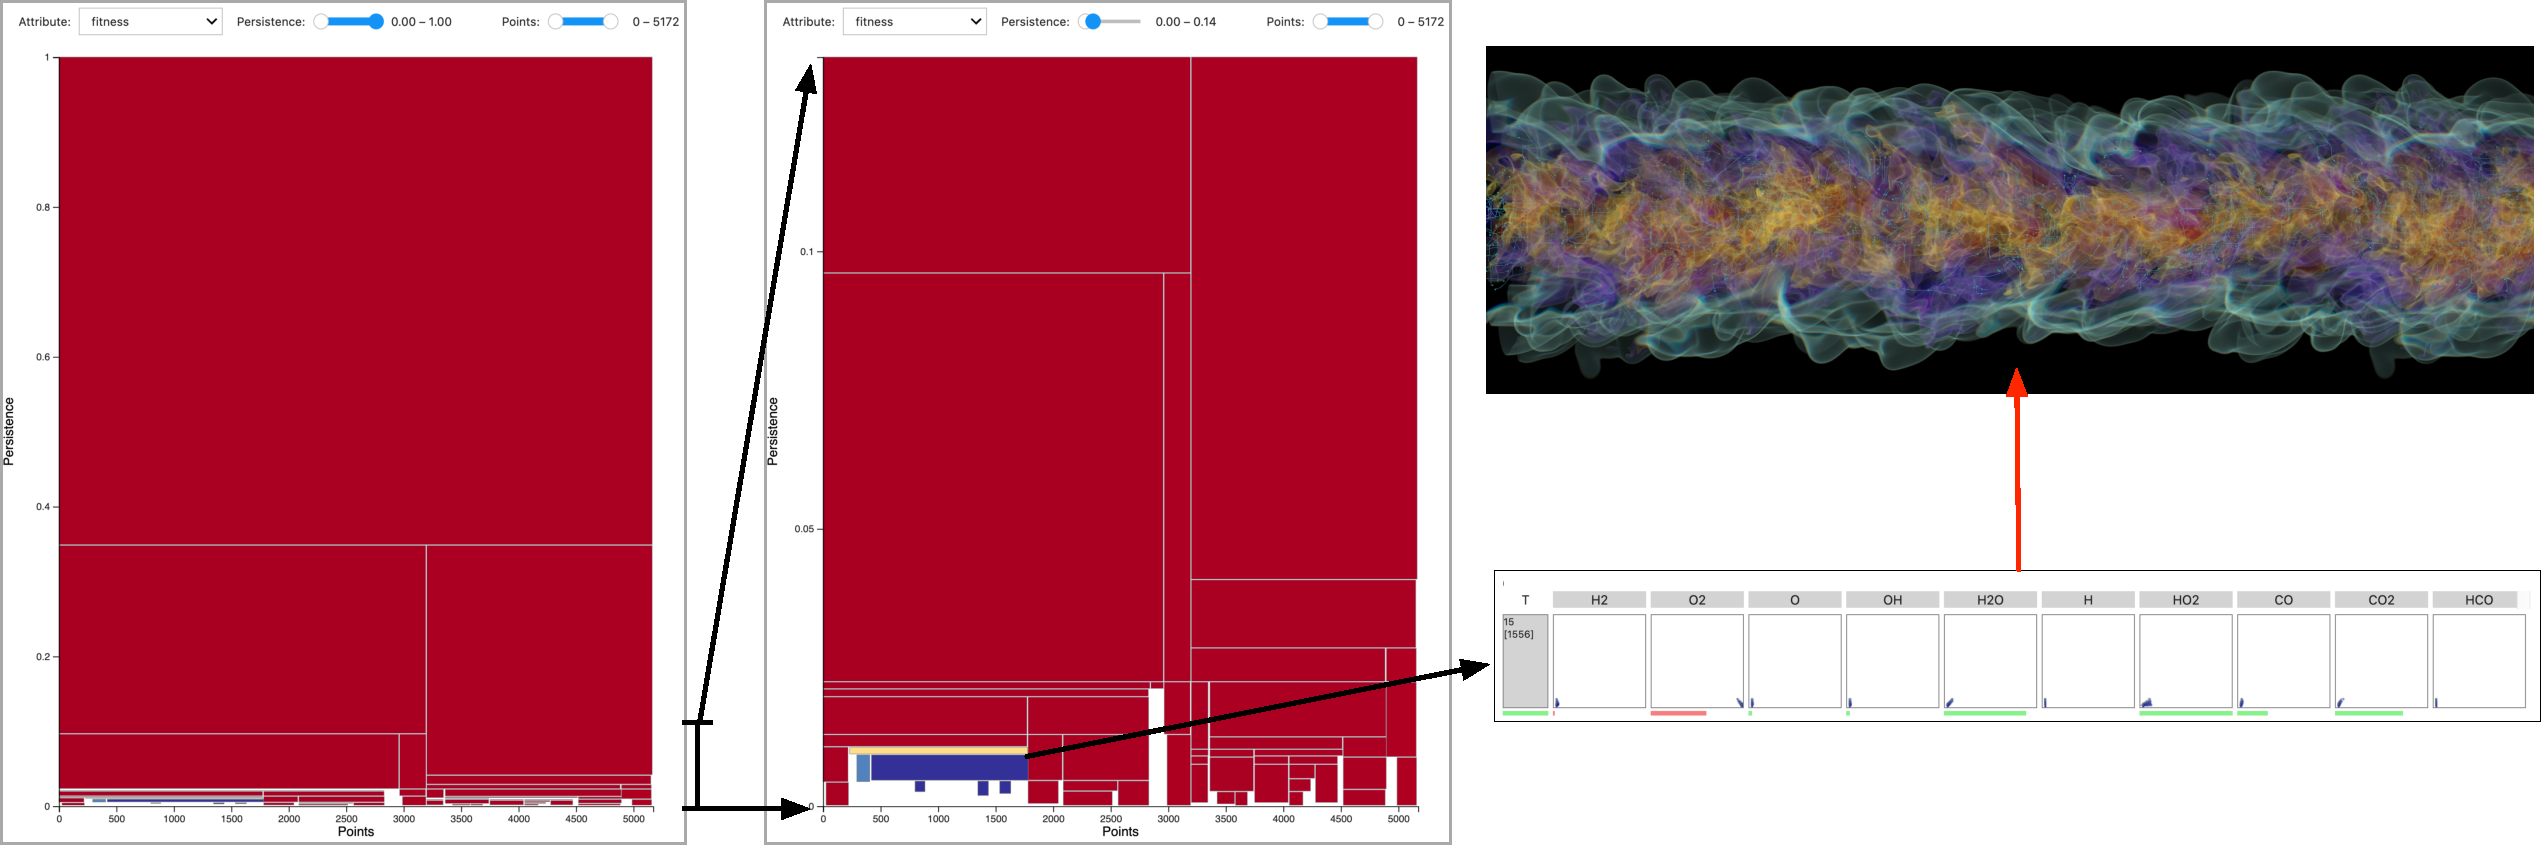
\includegraphics[width=\linewidth]{combustion-init-2}
     \vspace{-.2in}
    \caption{Combustion: Initial tree (left) shows that a single linear model describes all the data points(score = 0.998). Right: a zoom to persistence range [0:0.15] reveal a previously unknown partition containing large number (~30\%) of sample points that are outside of the active combustion zone and should have been removed (top).}
    \label{fig:combustion-init}
    \end{center}
         \vspace{-.1in}
\end{figure}

Using child and parent fitness doesn't reveal much but once we switch to child dimension fitness the tree comes to life, \autoref{fig:teaser}. The figure also shows the data points of the (four) top-most partitions that are different than their parents. Partition 494 (right most in the tree, bottom in the grid) is distinctly different from the other partitions. The three other partitions  differ mainly with respect of HO2, though the points in the first and third partitions (5 and 488) are mostly in the lower value. \autoref{fig:combustion-projections} shows the critical points graph. Note that the edges for the first three partitions overlap in (b) but are clearly separated in (c). 

The four partitions share a single maxima but feature four distinct minima. The minima in partition 494 captures a situation where fuel (H2 and CO) is available but the lack of oxidizer (O2) prevents a chemical reaction. The situation is reversed in partition 5 where oxidizer (O2) is available but the lack of fuel prevents a reaction. In partitions 460 and 488, the mixing of fuel and oxidizer is highly turbulent and blows the flames out, resulting in large amount of HO2. The clear separation between these two minima could be due to undersampling or possible the boundary of the manifold. 

% Originally only two minima were known and the third was discovered in an earlier work. The black annotation curve in (d) marks a possible boundary of the manifold, which may explain the three distinct minima we find in this area. The notches in this boundary, however, could also be due to undersampling. In contrast to the earlier work where the third minima was discovered after an exhaustive search through many potential simplifications and possible partitions, we were able to discover all four minima after a just a few steps in addition to identifying the invalid points. 

\begin{figure}[tb]
    \begin{center}
     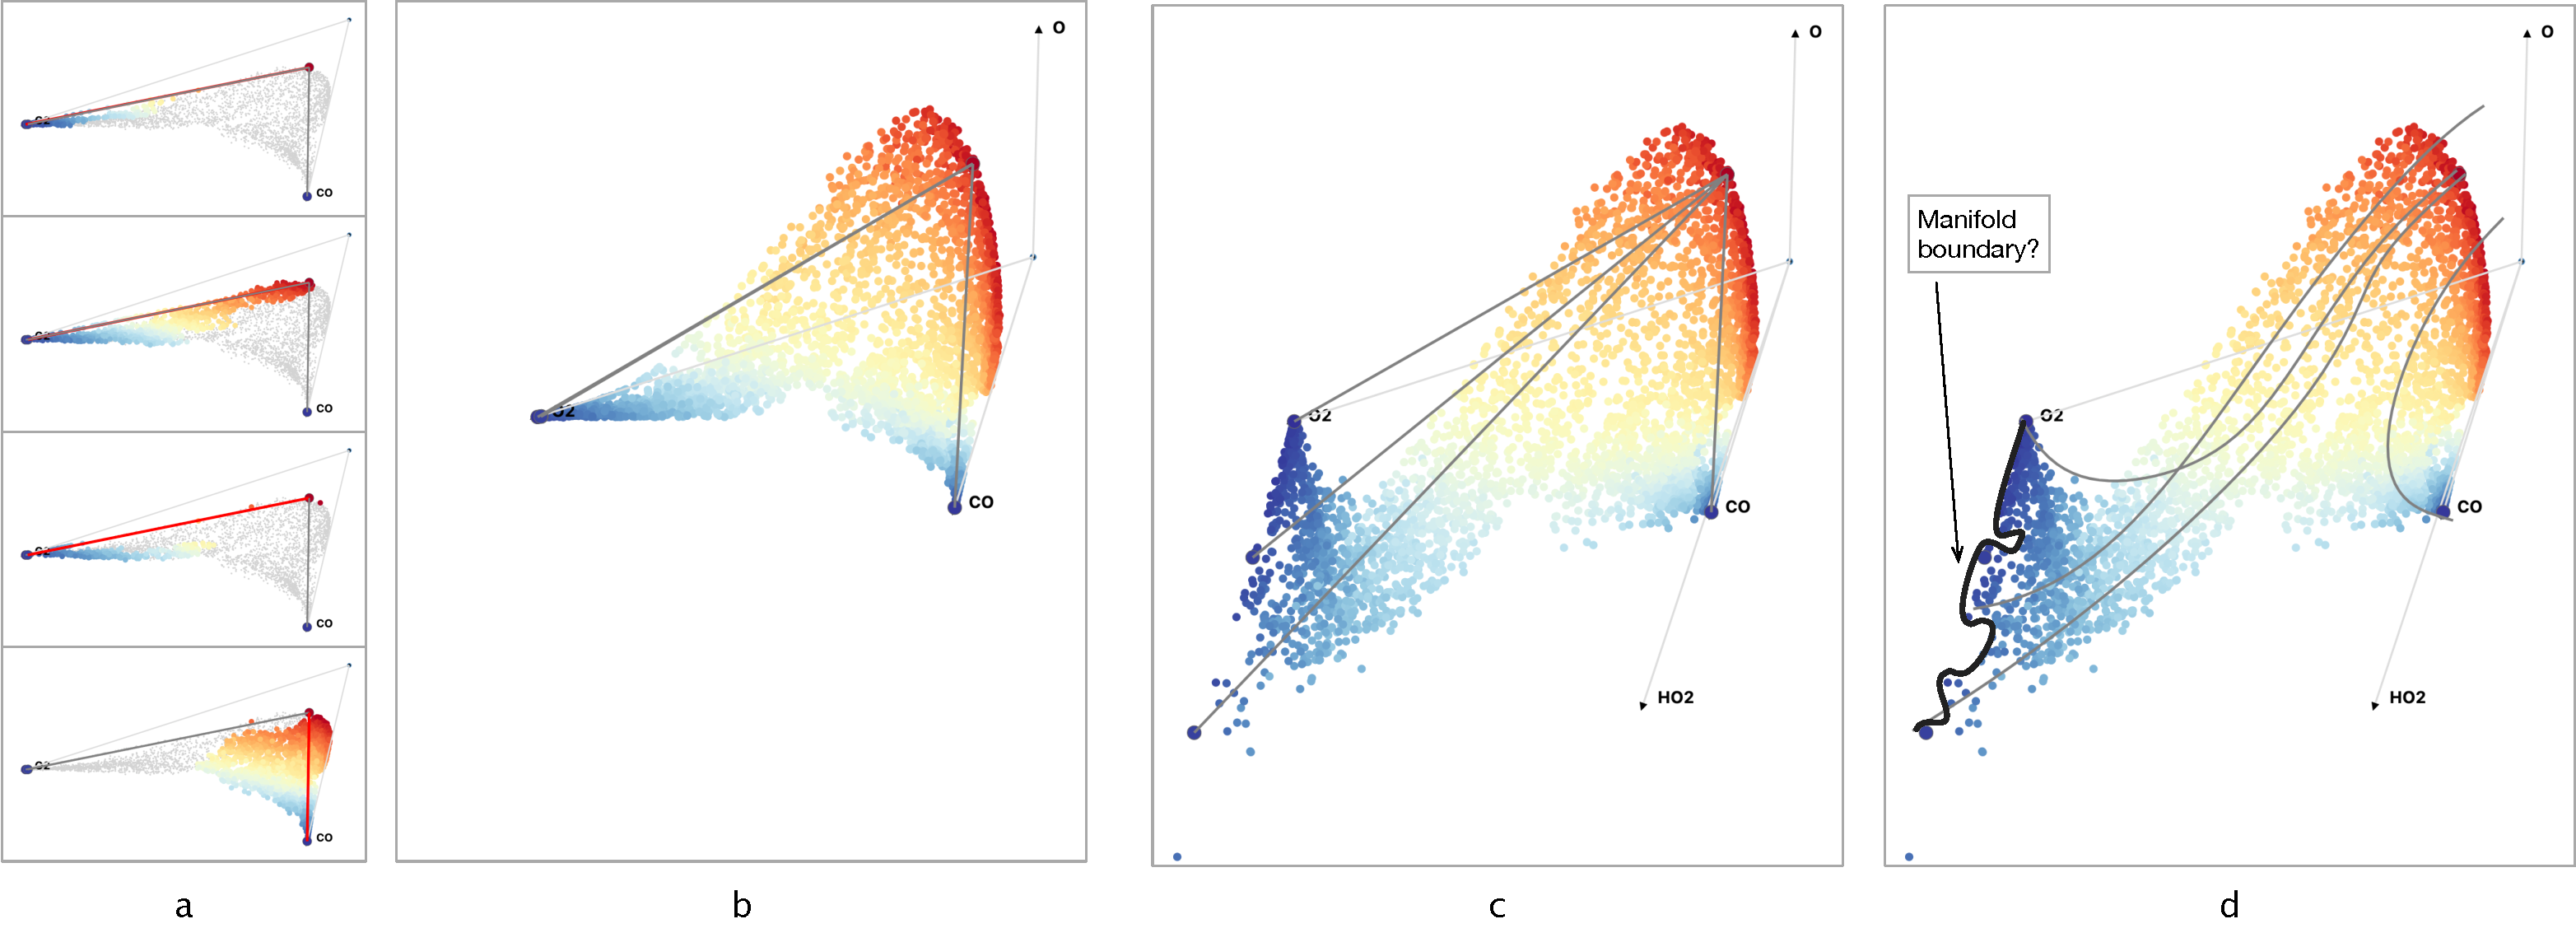
\includegraphics[width=\linewidth]{combustion-projections2}
             \vspace{-.1in}
    \caption{Graph views of the combustion data. a) Highlighting the points of each partition. b) Without the HO2 only the two expected minima are apparent. c) The three minima separates along the HO2 direction. d) Regression curves follow the shape of the manifold.}
    \label{fig:combustion-projections}
         \vspace{-.1in}
         \end{center}
\end{figure}

\subsection{Nuclear Fuel Cycle Simulations}
\label{sec:nuclear}
Nuclear fuel cycle analysis focuses on modeling the nuclear industry and ecosystem at a macroscopic level. This example studies scenarios for transitioning from one technology, Light Water Reactors (LWR) to a newer Sodium-cooled Fast breeder Reactor (SFR) technology. LWR reactors can use either enriched uranium (UOX, Uranium Oxyde) or a mixture of Uranium and Plutonium (MOX, Mixed Oxyde) as fuel but produce Minor Actinides waste. Minor Actinides have a long lifetime and high activities, which make such wastes  difficult to deal with. In contrast, SFR reactors mainly use a mix of Natural Uranium and Plutonium as a fuel (MOX). The SFR reactors have the ability to breed Plutonium from the Uranium and energy production is based on the fission of the Plutonium. This breeding capability allows the fuel to stay longer in the fuel, reducing the amount of Minor Actinides ultimately present in the waste. Some combination of fuel and SFR reactor configuration allows to breed more Plutonium than it will burn . A sufficiently large number of SFR reactors (used in 'breeder' configuration) can thus be self sustained.

\begin{figure}[b]
    \begin{center}
     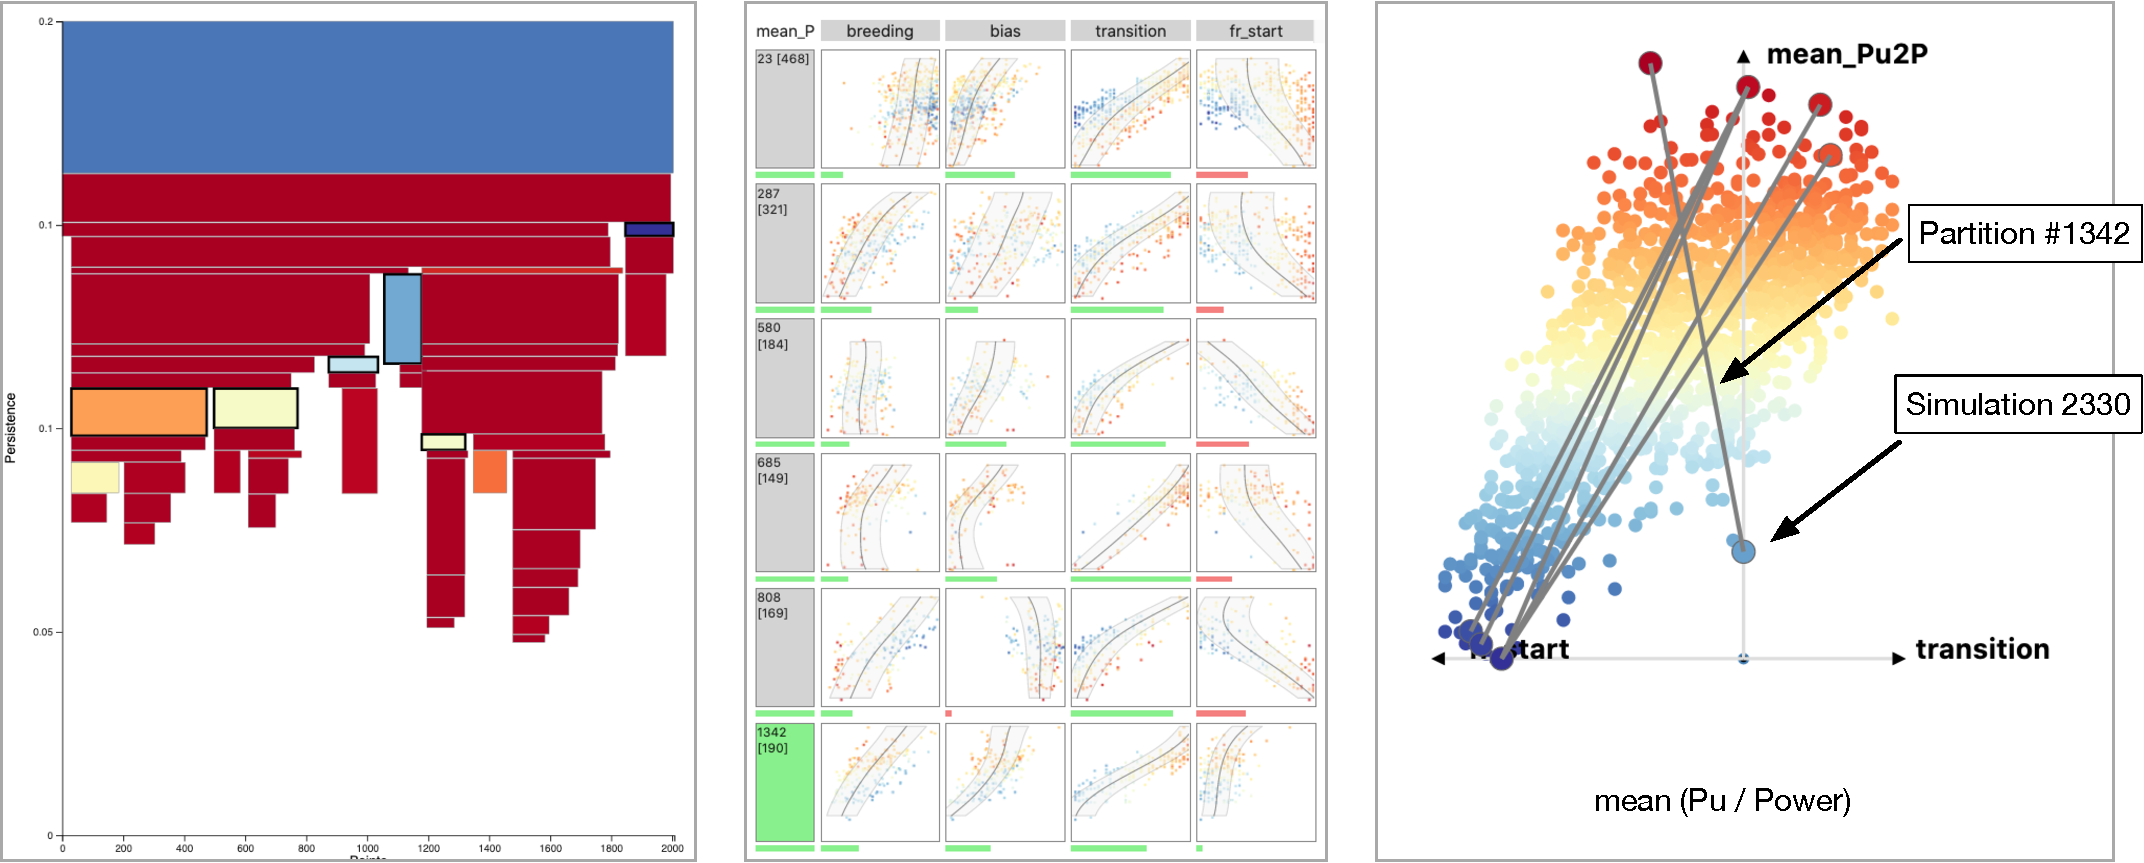
\includegraphics[width=\linewidth]{transition1}
    \caption{Transition scenario: Partitions selected based on dimension fitness (left). Partition 1342 exhibits unique behaviour (mid and right) though its minimum (simulation 2330) is not the lowest (right).}
        \vspace{-.1in}
    \label{fig:transition}
    \end{center}
\end{figure}

\begin{figure}[tb]
    \begin{center}
    \vspace{-.1in}
     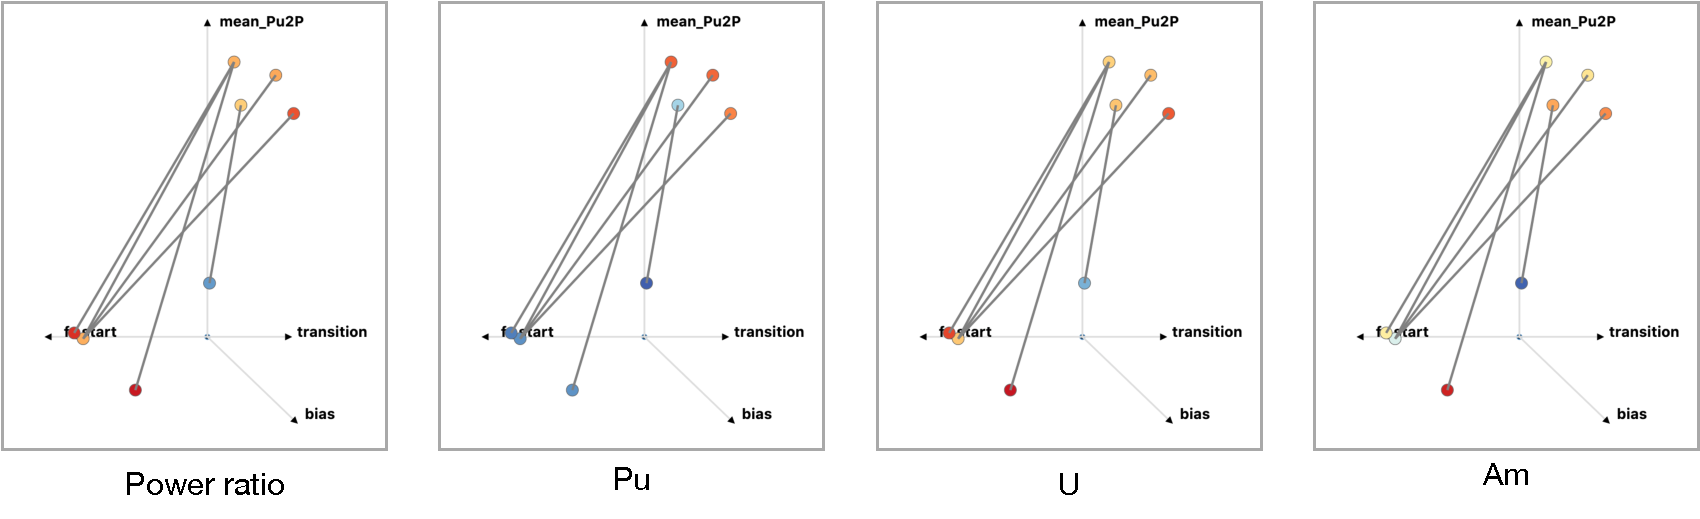
\includegraphics[width=\linewidth]{transition-graph1}
    \caption{Encoding other output variables as color demonstrates the advantages of simulation 2330 which exhibits low power ration and consistently generates low volumes of excess radio active materials.}
    \label{fig:transition-graph}
    \end{center}
\end{figure}

\begin{figure}[tb]
    \begin{center}
     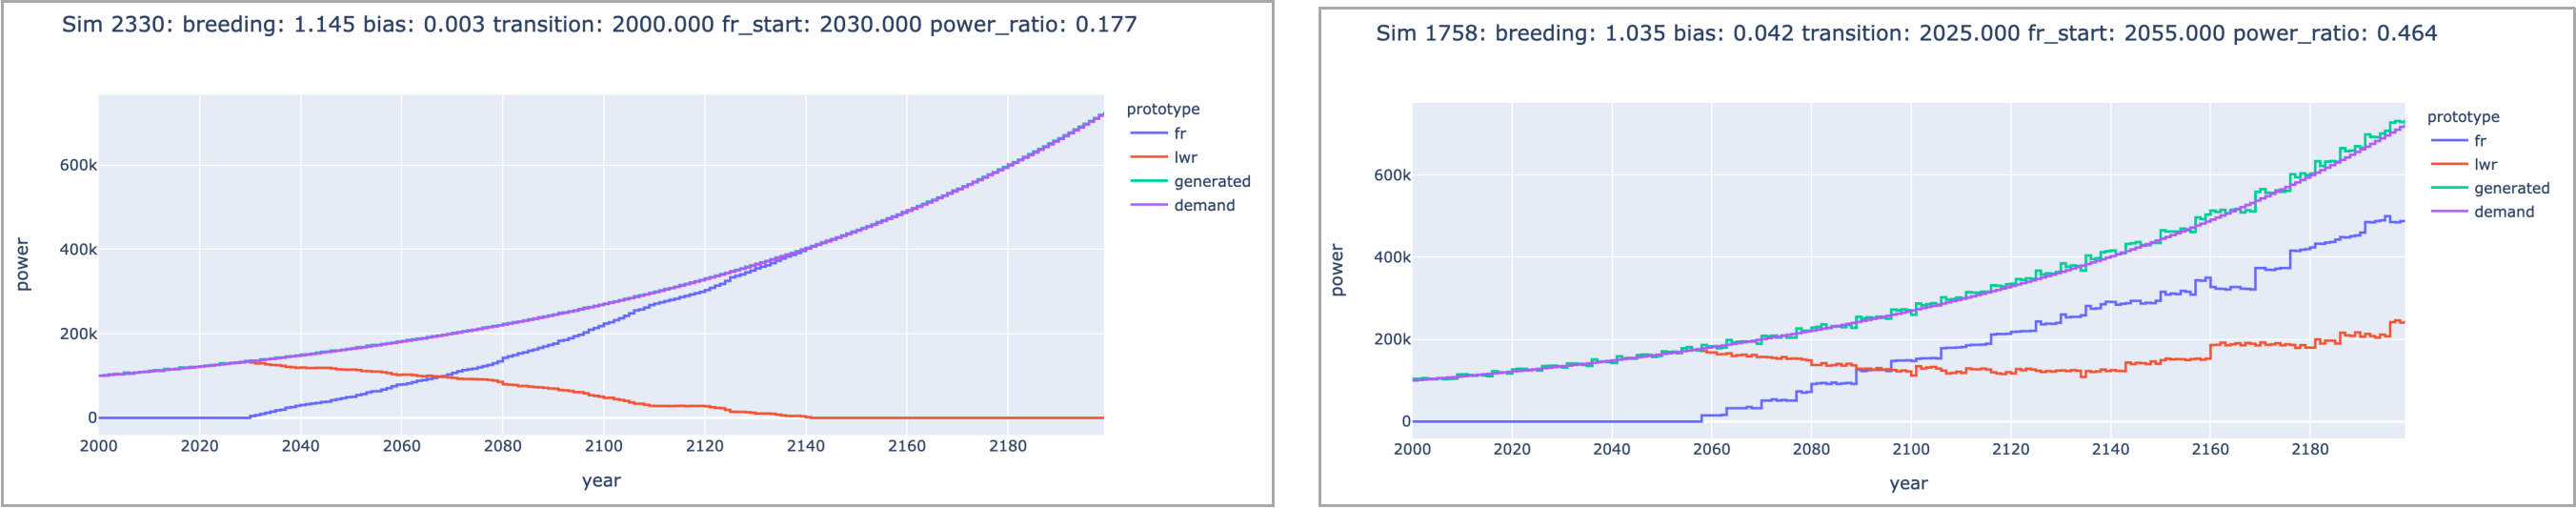
\includegraphics[width=\linewidth]{transition-plots-1}
    \caption{Simulation 2330 exhibits an excellent and smooth transition (left), while simulation 1758 does not lead to a transition (right).}
    \label{fig:transition-plots}
    \end{center}
\end{figure}

The study consists of 3300 simulation runs, using four input parameters (breeding ratio, start year of LWR fuel reprocessing, first year an SFR can be deploy and a bias measure). The aim here is to find a deployment schedule that transitions from an ecosystem consisting of LWRs to one with only SFR reactors, while minimizing some objective function. To this end we computed several objective functions at the end of each simulation including: the ratio of total power generated by LWRs reactors to the total energy generated over the simulation's 200 years span, the mean ratio of plutonium to generated power, and amount of nuclear waste such as Plutonium, Uranium and Americium. 
Of the 3300 simulation only 2007 led to a complete transition within the first 120 years). In the following we looked at the mean ration of Plutonium to power objective function. \autoref{fig:transition} show a reduced \RT (remove partitions with less than 100 simulations or a lifespan less then 0.001) depicting child dimension fitness. Several partitions that stand out are also shown. The graph view on the right shows that partition 1342 exhibits a unique behaviour, although its minima (simulation run 2330) doesn't have the lower value. \autoref{fig:transition-graph} shows that adding 'bias' in the graph view affects only one of the minima. However, when we use the same partitions and graph, but change the colors to encode other output values, we can see that simulation 2330 is unique in that it consistently exhibits low values (blues) for power ration and the amount of the nuclear waste generated. \autoref{fig:transition-plots} shows the deployment schedule of simulation 2330 (top) and an example of a simulation that doesn't lead to a complete transition. 
 


% \todo[inline]{Linear models in multi-dimensional may not be intuitive, for example the fr\_start in the transition use-case}
\section{Conclusions}
\label{sec:conclusions}
The \RT addresses the important, though often neglected, 'why' question by  proposing a new perspective of the topology simplification process. The \RT visualization offers both a concise broad view of the simplification landscape and a guide for an interactive visual exploration of the underlying scalar function. We describe the \RT in the context of Morse-Smale complexes, but the partition's perspective and the tree are equally applicable to Morse complexes. Some of the measures as well as the inverse regression curves are not directly applicable and one will have to use high order regression models.

The \RT has several limitations. First, it does not preserve spatial locality or even adjacency relation between partitions. Mapping spatial locality is a complex issue for multi-dimensional data in general. Adjacency information can be retrieved from the Morse-Smale complexes, though how to depict it is not clear and is especially problematic in a setting with many levels of details. 
Second, Morse-Smale partitions can have complex twisting shapes that are not captured directly in the tree structure and the tree does not address the notion of topological holes. 

We have begun exploring methods for using the inverse regression curves to facilitate adaptive sampling, both for validation purposes and for improving spatial resolutions in areas that are undersampled. We are also looking at using t-SNE and other dimensional reduction and clustering techniques to analyze the linear models and provide additional measures for identifying and highlighting potential unique partitions.

% \section{Acknowledgments}
% This work was funded in part by the U.S. Department of Energy, Nuclear Energy University Program (NEUP) grant DE-NE0008587.


%% if specified like this the section will be committed in review mode
\acknowledgments{
The authors wish to thank A, B, and C. This work was supported in part by
a grant from XYZ (\# 12345-67890).}

%\bibliographystyle{abbrv}
\bibliographystyle{abbrv-doi}
%\bibliographystyle{abbrv-doi-narrow}
%\bibliographystyle{abbrv-doi-hyperref}
%\bibliographystyle{abbrv-doi-hyperref-narrow}

\bibliography{paper,ondemandaccurate,vis2014}
\end{document}
